\documentclass[letterpaper, 10pt, conference]{IEEEtran}
\usepackage{times}
\usepackage{xr}
\usepackage{amsmath,amssymb,mathrsfs}
\usepackage[]{algorithm2e}
\usepackage{graphicx}
\usepackage[table]{xcolor}
\usepackage{wrapfig}
\usepackage{textcomp}
\usepackage{booktabs}
\usepackage{multirow}
\usepackage{textcomp}
% \usepackage[T1]{fontenc}  % double sans serif quotation
\usepackage{textcomp} % single
% \usepackage{titling}

\definecolor{control}{RGB}{203, 65, 107}
\definecolor{shape}{RGB}{61, 153, 115}

% \usepackage{setspace}
% \doublespacing

% numbers option provides compact numerical references in the text. 
\usepackage[numbers]{natbib}
\usepackage{multicol}
\usepackage[bookmarks=true, hidelinks, colorlinks = true, linkcolor = black, urlcolor  = blue, citecolor = black, linkcolor=black]{hyperref}

\begin{document}

% paper title
\title{\vspace{5pt}Scalable sim-to-real transfer of soft robot designs}

% You will get a Paper-ID when submitting a pdf file to the conference system
\author{Author Names Omitted for Anonymous Review. Paper-ID [add your ID here]}


% avoiding spaces at the end of the author lines is not a problem with
% conference papers because we don't use \thanks or \IEEEmembership


\author{
\IEEEauthorblockN{Sam Kriegman$^1$,\quad
Amir Mohammadi Nasab$^2$,\quad
Dylan Shah$^2$,\quad
Hannah Steele$^2$,\quad
Gabrielle Branin$^2$,\\[2pt]
Michael Levin$^3$,\quad
Josh Bongard$^1$,\quad
Rebecca Kramer-Bottiglio$^2$}\vspace{6pt}%\vspace{4pt}
\IEEEauthorblockA{$^1$University of Vermont,  $^2$Yale University,  $^3$Tufts University}
}



\teaser{
\centering
\vspace{-6pt}
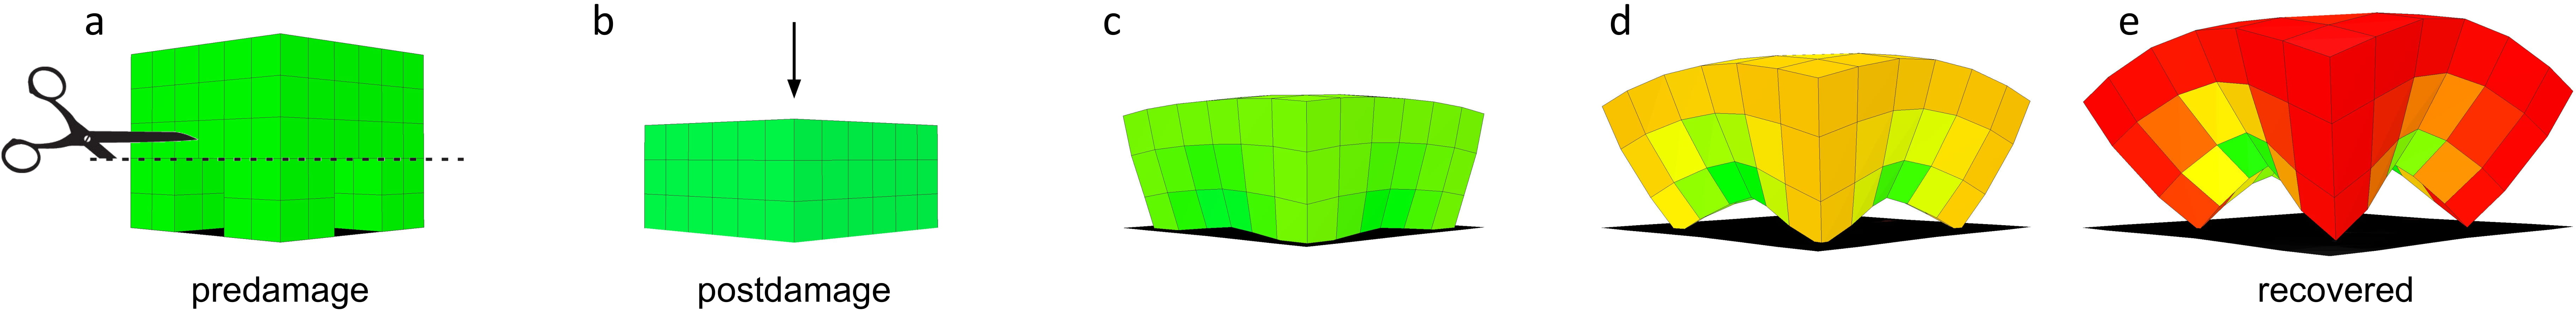
\includegraphics[width=\linewidth]{fig/bigger_teaser.jpg} \\
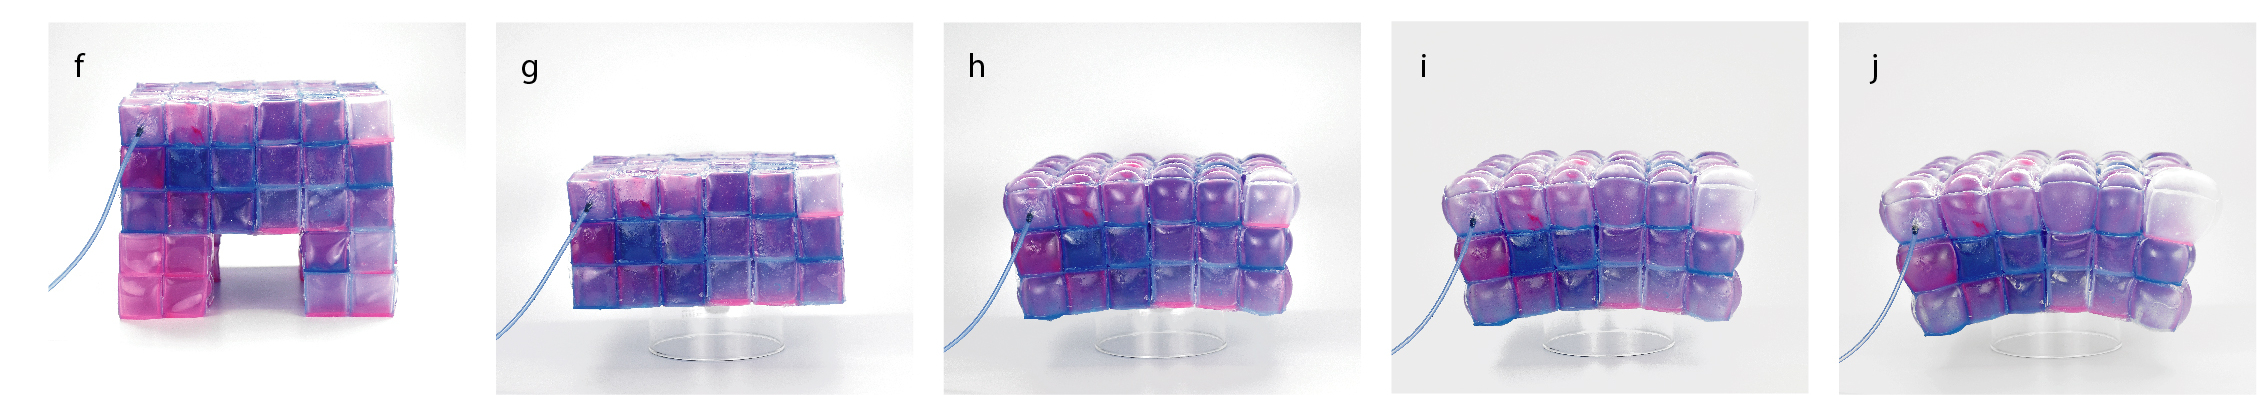
\includegraphics[trim={0 0 0 4pt},clip,width=\linewidth]{fig/VoxelBotCropped.jpg} \\
\vspace{-4pt}
\caption{After learning to walk, a simulated quadruped is subjected to unanticipated insult: its legs are cut off. 
An evolutionary algorithm searches for deformations to the postdamage structure that, when coupled with the predamage controller, result in function recovery.
One of the evolved solutions (shown here) yields the spontaneous ``regeneration'' of the lost legs, which was manually transferred to reality (\href{https://youtu.be/afOXX2r54mQ}{\textcolor{blue}{\textbf{\texttt{youtu.be/afOXX2r54mQ}}}}).
} 
\label{fig5:teaser}
\vspace{-20pt}
}




\maketitle

\begin{abstract}
% 
\noindent
A robot's mechanical parts routinely wear out from normal functioning and can be lost to injury. For autonomous robots operating in isolated or hostile environments, repair from a human operator is often not possible.
Thus, much work has sought to automate damage recovery in robots.
However, every case reported in the literature to date has accepted the damaged mechanical structure as fixed, and focused on learning new ways to control it.
Here we show for the first time a robot that automatically recovers from unexpected damage by deforming its resting mechanical structure without changing its control policy.
We found that, especially in the case of ``deep insult'', such as removal of all four of the robot's legs, the damaged machine evolves shape changes that not only recover the original level of function (locomotion) as before, but can in fact surpass the original level of performance (speed).
This suggests that shape change, instead of control readaptation, may be a better method to recover function after damage in some cases.
%

\end{abstract}

\IEEEpeerreviewmaketitle

\section{Introduction}
\label{sec5:intro}


Certain remote, hazardous or otherwise inaccessible environments preclude human intervention when a robot fails or is damaged.
It would thus be advantageous for systems operating in such environments to have some capacity for self -maintenance and -repair.


Indeed, much work has investigated how,
in the absence of external supervision,
a robot can automatically learn new ways to control its body when damaged~\mbox{\cite{bongard2006resilient, chatzilygeroudis2018reset, cully2015robots, kano2017brittle, kwiatkowski2019task, mahdavi2003evolutionary, ren2015multiple}.}
While a diverse set of recovery mechanisms have been proposed, they all  
shared a common assumption: 
The damaged mechanical structure could be 
reconfigured, but not fundamentally deformed.


This assumption is reasonable in classical robots, which are, generally, jointed collections of rigid links.
But recent advances in materials science and 3D printing are enabling the construction of soft machines with theoretically infinite degrees of freedom and thus capable of deforming their
structures so as to regenerate a lost part or embrace an entirely new geometry in the face of unanticipated insult. 
The possibility of such change affords a completely novel mode of damage recovery:
No robot built to date has altered its resting structure in order to recover function lost due to damage.


Previous computational studies have demonstrated structural but non-functional change in discrete models.
For example, cellular automata have been trained to grow a target structure from a single cell \cite{eggenberger1997evolving, miller2004evolving}.
Similar growth rules could in principle be instantiated in self-assembling modular robots~\cite{white2005three,zykov2005robotics}.
However, structural change would require access to additional modules in the environment, redundant modules on the body, or the ability to internally generate them.
Moreover, it is unclear how or if such rules could dictate continuous geometric deformation in soft robots.

The present work builds on two closely-related research projects in which injured robots automatically generate and test candidate control policies in order to find compensatory behaviors that work in spite of damage
\cite{bongard2006resilient,cully2015robots}.



In the first, \citet{bongard2006resilient} demonstrated how, under the right conditions, an autonomous robot could internally model its own geometry with minimal sensorimotor experiment.
The benefit of this approach is that, once a sufficiently accurate self-model has been established, actions can be internally rehearsed, discarding those which are unsuccessful or dangerous, before attempting them in reality.
If model accuracy drops, as from structural changes due to damage, modeling resumes and continues until the robot's current morphology is adequately reflected in the robot's model of self.

The main drawback of this approach is that internal modeling requires additional computation, and there are circumstances in which the robot cannot afford---in terms of time, money, energy, stability, and the overall well-being of itself and others---to remain stationary for extended periods of time.

To speed recovery, \citet{cully2015robots} proposed that robots should instead exploit the fact that resources prior to deployment are relatively cheap in terms of the factors listed above.
A large, behavioral repertoire composed of mappings from behaviors (for the undamaged robot) to their predicted performances can therefore be modeled in simulation beforehand, and come preinstalled on the robot.
Assuming damage is detected by an external mechanism, the authors showed how, under certain conditions, such a map can be rapidly updated and traversed to find successful behavior, 
which is 
implicitly robust to differences between the current and pre-deployment
morphologies.



The robots used in this past work consisted of rigid components attached together with a handful of mechanical degrees of freedom:
The quadruped in \cite{bongard2006resilient} had 8 motors and 4 DOF; 
the hexapod in \cite{cully2015robots} had 18 motors and 12 DOF.
The control problem was greatly impacted by these mechanical details and their intrinsic dynamics, but they were taken as given, even when damaged, because these robots simply could not deform their resting structure.


Instead of treating the body as just the problem domain, we here modify it as part of the computational loop.
This is possible because our robot has many more (140) mechanical degrees of freedom, and the ability to change the volume, rather than just the relative displacement, of each component.
This flexibility enables a heretofore unexplored mode of damage recovery: keep the existing controller but deform the resting structure.
Existing approaches to controller adaptation could in principle (although this is not investigated here) be paired with such changes to morphology.
However, in many cases, it would be desirable to retain a previously optimized and fine-tuned controller, especially if missing structure can simply be regenerated.

We here show that, under a wide range of damage scenarios, automated shapeshifting can be advantageous, and that, in most of the cases tested, shapeshifting alone (holding the existing controller fixed) outperforms controller adaptation alone (holding the damaged shape fixed), in terms of recovered mobility.





\begin{table}[t]
\footnotesize
\caption{\label{table:lit_review}Summary of published sim2real transference.}
\vspace{-1.25em}
\begin{center}
\begin{tabular}{lccc} 
    \toprule
    \textit{Author/citation} & \textit{Year} & \textit{Controllers} & \textit{Morphologies} \\ 
    \midrule
    % \citet{cliff1993explorations}   & 1993 & 1 & 1 \\ % no data from real robot was reported.
    
    \citet{Miglino1994Selection}    & 1994 & 1 & 1 \\  % lego wheeled bot
    \citet{jakobi1995noise}         & 1995 & 2 & 1 \\  % Khepera: light seeking and obstacle avoidance.
    
    % \citet{miglino1995evolving}     & 1995 & 1 & 1 \\ % Khepera obstacle-avoidance (while moving forward as fast as possible, moving in as straight a line as possible, and keeping as far away from objects as possible) (one fitness function).
    
    \citet{HARVEY1997205}           & 1997 & 4 & 1 \\  % Jakobi's previously repoted Khepera results but also new Gantry results: forward movement, move toward small object, move toward large object, classify triangle vs square
    
    \citet{lipson2000automatic}     & 2000 & 3 & 3 \\
    
    \citet{bongard2006resilient}    & 2006 & 34 & 2 \\
    
    \citet{hiller2011automatic}     & 2011 & 1 & 5 \\ 
    
    \citet{koos2012transferability} & 2012 & 2 & 2 \\ 
    
    \citet{moeckel2013gait}         & 2013 & 1 & 1 \\  % gaits for a modular robot snake (structure fixed) 
    
    \citet{caluwaerts2014design}    & 2014 & 2 & 1 \\ % spherical tensegrity locomotion: a hand designed controller (releasing tensioned springs) and a feedback controller (Matsuoka oscillator)
    
    \citet{cully2015robots}         & 2015 & 10 & 10 \\
    
    \citet{cellucci20171d}          & 2017 & 1 & 3 \\
    
    \citet{tobin2017domain}         & 2017 & 1 & 1 \\ % visual object detector 
    
    % \citet{james2017transferring}   & 2017 & 1 & 1 \\ % pickup and place a cube in a basket  % domain randomization
    
    \citet{rusu2017sim}             & 2017 & 1 & 1 \\ % reaching a visual target
    
    \citet{peng2018sim}             & 2018 & 1 & 1 \\ % push a puck
    % \citet{sadeghi2018sim2real}     & 2018 & 1 & 1 \\ % reaching  % visual servoing
    
    \citet{Pinto-RSS-18}            & 2018 & 3 & 1 \\ % pick, forward push, block move % asymmetric actor critic
    
    \citet{tan2018sim}              & 2018 & 2 & 1 \\ % trotting and galloping
    
    % \citet{bharadhwaj2018data}      & 2018 & 1 & 1 \\ % visual tiny car navigation in duckytown
    
    \citet{pmlr-v87-golemo18a}      & 2018 & 1 & 1 \\ % sword vs shield fight  % neural augmented sim
    
    \citet{matas2018sim}            & 2018 & 3 & 1 \\ % folding a towel up to a mark, folding a face towel diagonally, and draping a piece of cloth over a hanger.
    
    % \citet{tobin2018domain}         & 2018 & 1 & 1 \\ % grasping (procedurally generated objects; domain randomization)
    
    % \citet{collins2019quantifying}  & 2019 & 1 & 1 \\ % quantifying the reality gap for 5 physics engines and a robot arm
    
    % \citet{chebotar2019closing}     & 2019 & 2 & 1 \\ % opening a cabinet drawer and swinging peg-in-hole  % domain randomization applied according to interactions with reality
    
    \citet{kwiatkowski2019task}     & 2019 & 2 & 2 \\
    
    \citet{hwangbo2019learning}     & 2019 & 3 & 1 \\ % commanded locomotion, high-speed locomotion, recovery from fall
    
    \citet{kriegman2019automated}   & 2019 & 1 & 5 \\
    
    \citet{nachum2019multi}         & 2019 & 3 & 1 \\  % avoid, push, coordinate
    
    \citet{akkaya2019solving}       & 2019 & 1 & 1 \\
    
    \citet{rosser2019sim2real}      & 2019 & 1 & 16 \\
    
    \textbf{The results presented here} & \textbf{2019} & \textbf{1} & \textbf{108} \\
    \bottomrule
\end{tabular}
\end{center}
\vspace{-1.75em}
\end{table}



\section{Methods}
\label{sec:methods}

This section describes the hardware, simulation and control of our robot,
the damage scenarios it faces and its options for recovery: 
shapeshifting and controller adaptation.
We also define a tripartite classification|of `structure', `shape' and `configuration'|that forms the basis of our argument, which is, briefly, that the way in which our robot recovers from damage|shape change|was outside the scope of any robot previously reported in the literature.


\subsection{The source code.}
\href{https://github.com/skriegman/2019-RSS}{\textcolor{blue}{\textbf{\texttt{github.com/skriegman/2019-RSS}}}}



\subsection{The robot.}
\label{sec:robot}


The robot is an isobilaterally symmetrical quadruped constructed from 140 inflatable silicone ``voxels'' 
(Figs.~\ref{fig:teaser}f and~\ref{fig:blue_quad}).
We here present a method for creating air-filled voxel membranes with relatively uniform thickness.

% Blue VoxelBot
\begin{wrapfigure}{r}{0.4\linewidth}
\vspace{-14pt}
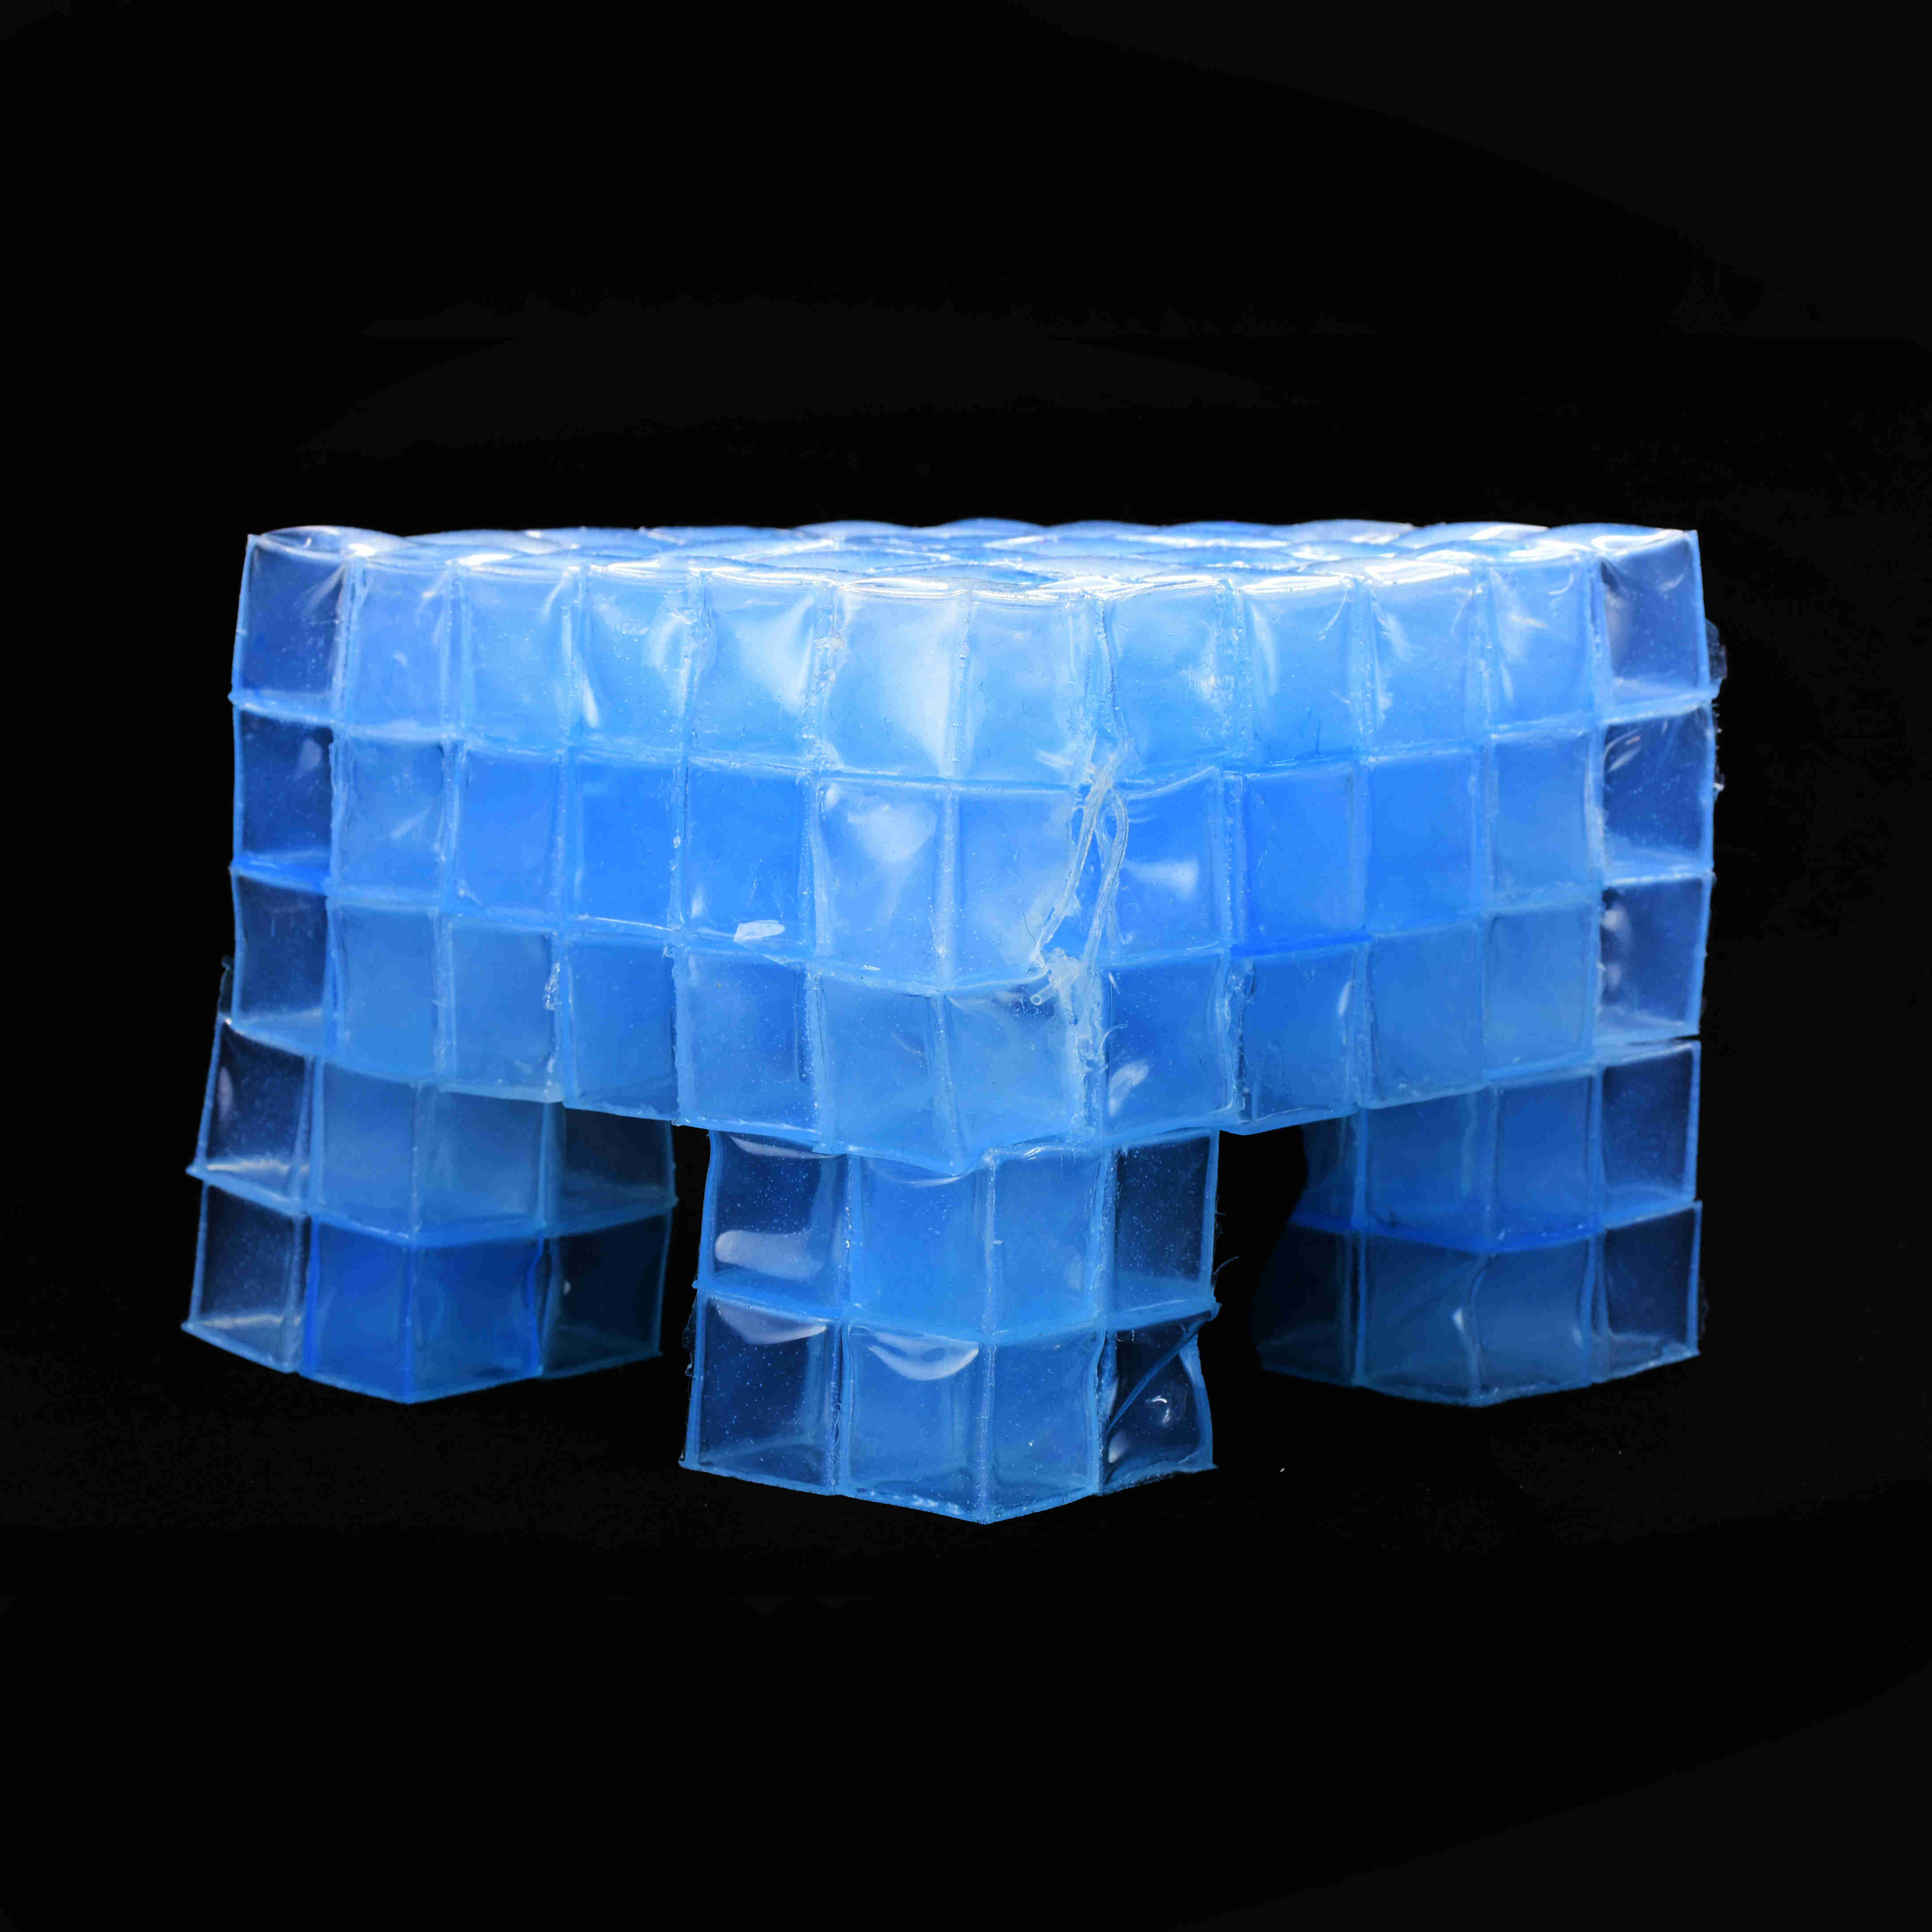
\includegraphics[trim={0 16em 0 17em},clip,width=\linewidth]{Chapter05/fig/DSC_8734_crop-min.jpg}
\vspace{-18pt}
\caption{The blue robot, made from thin-walled inflatable elastomer voxels.}
\label{fig5:blue_quad}
\vspace{-1em}
\end{wrapfigure}



Creating thin, hollow 3D silicone structures is challenging due to several factors, including mold precision and potential for damage during release from molds. One effective but labor-intensive method is to make the 3D shapes by adhering 2D films at their joints \cite{morin_elastomeric_2014}. Here, inspired by a scalable 2-axis rotational molding technique \cite{zhao_scalable_2015}, we employ a \mbox{1-axis} rotational drip-molding machine.

First, silicone (Dragon Skin 10 Fast; Smooth-On, Inc.) was poured into an open-face acrylic mold and a tongue depressor was used to roughly spread the silicone along the walls. The mold was then attached to the rotational molding machine with the rotation axis oriented downward at 45 degrees relative to horizontal, and run through cycles comprising a 90\textdegree~turn, stopping for 45 seconds after each turn to allow the silicone to flow and evenly coat each side. Excess silicone dripped out of the mold, leaving a thickness which was dependent on several interrelated factors including the cure time, viscosity, and the interaction between the silicone and acrylic.

After the silicone cured, excess material was cut away. A silicone base-layer was then rod-coated onto a flat acrylic sheet. Next, the bottomless cubes were placed on the base-layer and allowed to cure, sealing air inside each voxel. The voxels were then cut from the sheet and a small hole was punched in each voxel for tubing. Finally, silicone tubes were inserted and bonded with Sil-Poxy (Smooth-On, Inc.).

The overall robot consists of a $6\times6\times3$ voxel torso and four removable $2\times2\times2$ voxel legs (Figs.~\ref{fig:teaser}f-j  and~\ref{fig:blue_quad}). 
Sil-Poxy and Ecoflex 00-50 were used to improve adhesion between voxels. 
To explore the effect of layer thickness on the range of attainable morphologies,
two versions of the robot were fabricated:
The {\color{blue}\textbf{blue robot}} (Fig.~\ref{fig:blue_quad}) consists of voxels made with one layer of silicone, while the {\color{purple}\textbf{purple robot}} \mbox{(Fig.~\ref{fig:teaser}f-j)} consists of thicker-walled voxels made with two layers of silicone. 

Individual cubic voxels were manually inflated at pressures less than 20~kPa, and approached a spherical shape as pressure increased. 
When patterned together into a robot, selective inflation of a subset of voxels induces overall robot shape change. 
To reduce friction and weight effects in the robots, they were placed on top of a glass crystallizing dish, which lifted their legs off the table surface.
While this arrangement made motion difficult, it allowed us to conduct a preliminary investigation of the feasibility of transferring simulated shape change to a physical system. 
In future implementations, the manual inflation could be replaced by pressure regulators~\cite{booth_addressable_2018}, allowing the robot to approach the continuous control achievable in simulation.

To understand some of the trade-offs between design parameters, consider a spherical pressure vessel in uniform free expansion:
\begin{equation}
    \label{eq:pressure vessel}
    p=\frac{2 E \cdot \epsilon \cdot t}{r} = \frac{2 E \cdot \epsilon \cdot t_0 \cdot (1-\delta)}{r_0-\epsilon},
\end{equation}
where $t_0$ [m] is the thickness of the pressure vessel, $r_0$~[m] is the radius, $\epsilon$ is the linear strain due to expansion, $E$ [MPa] is Young's modulus, and $\delta$ is the radial strain (which is determined from $\epsilon$ and the material's Poisson's ratio).
Note that each voxel can push outward with a force proportional to the pressure. Examining Eq.~\ref{eq:pressure vessel}, we see that at a given strain rate and initial dimensions, the internal pressure scales linearly with both thickness and modulus. Thus, when choosing thickness of voxels, there was a tradeoff between weight and internal pressure: doubling the wall thickness doubled weight, in exchange for doubled operational pressure.



\subsection{The simulation.}

To simulate the robot, we use the voxel-based physics engine \textit{Voxelyze} \cite{hiller2014dynamic},
which simulates elastic voxels using two elements: particles and beams.
Particles have mass and rotational inertia, and are connected on a cartesian grid by spring-like beams (with translational and rotational stiffness).
For visualization and reference, part of a voxel mesh is drawn around this structure such that each voxel has a single particle at its center (Fig.~\ref{fig:voxcad}).

% \definecolor{darkgray}{HTML}{606060}
% \definecolor{darkblue}{HTML}{003366}
% \definecolor{darkred}{HTML}{990000}
\begin{wrapfigure}{r}{0.4\linewidth}
\vspace{-1em}
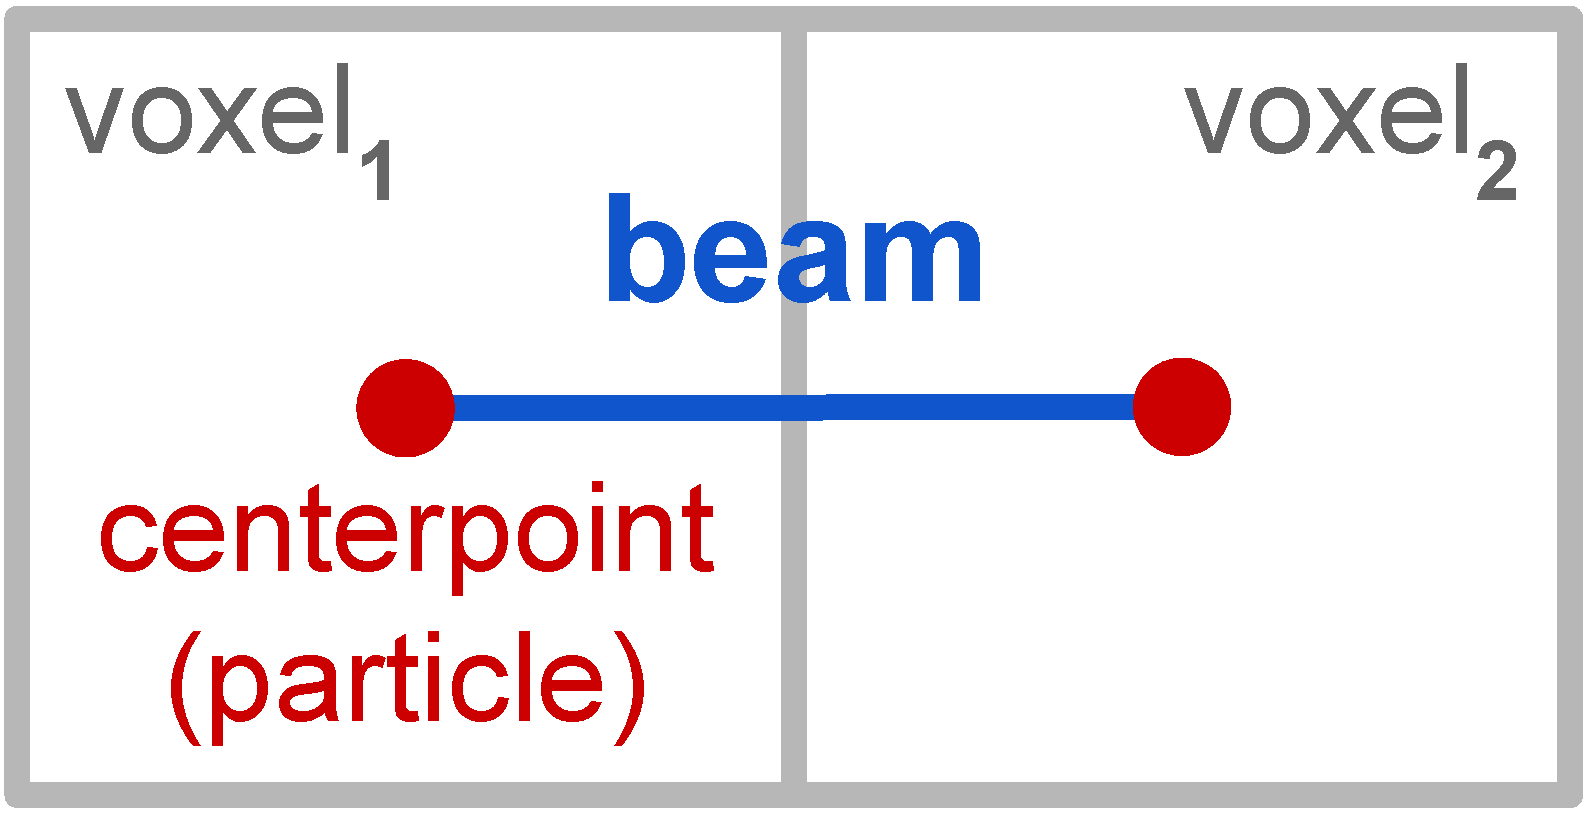
\includegraphics[trim={0 0 0 0},clip,width=\linewidth]{Chapter05/fig/two_cubes.pdf}\\
\vspace{-19pt}
\caption{Voxels are simulated by beams (springs) and particles (masses).
}
\label{fig:voxcad}
\vspace{-1em}
\end{wrapfigure}

Two adjacent voxels are connected, centerpoint to centerpoint (i.e.,~particle to particle), by a single, shared beam.
Material properties (e.g.,~volume and elasticity) are specified at the particles but implemented as attributes of beams (e.g.,~their rest length, and how easily they twist and stretch).
Where two adjacent particles disagree in their ``desired'' attributes of a shared beam, an average is taken.

A beam exits a voxel normal to, and in the center of, one of the voxel's faces.
Although the mesh is drawn such that voxel edges bend around the underlying beam-mass network (see,~e.g.,~Fig.~\ref{fig:teaser}), a spherical envelope is used for collision detection, thus approximating the spherical expansion of the physical voxels (with maximal expansion occurring at the center of each face).
For more details see \cite{hiller2014dynamic}.


\subsection{The structure and shape of a robot.}

The \textbf{structure}, $\mathbb{S}$,
of a robot is determined by the number and placement of voxels, and simulated by the presence and absence of particles on a regular grid in the workspace.
Let the bit value $v_i$ denote the presence ($v_i=1$) or absence ($v_i=0$) of a voxel at index~$i$.
The structure,
\begin{equation}
    \label{eq:structure}
    \mathbb{S} = \{i : v_i = 1 \} ,
\end{equation}
is thus a set of voxel coordinates.

The \textbf{shape}, $\mathcal{S}$,
of a robot is determined by the resting volume of each voxel, which is expressed in simulation as the resting (or, equilibrium) lengths of the beams connecting adjacent particles, and in reality as a resting pressure within each voxel (though the exact pressure, $p_i$, is not measured here).
Let the floating point value $b_i$ denote the beam rest length stored at the $i$-th simulated voxel.
The shape,
\begin{equation}
    \label{eq:shape}
    \mathcal{S}_{\text{sim}} = \{b_i : i \in \mathbb{S} \} \; \sim \; \mathcal{S}_{\text{real}} = \{p_i : i \in \mathbb{S} \} ,
\end{equation}
is thus a set of voxel resting volumes.

The robot has a quadrupedal predamage structure (Figs.~\ref{fig:teaser}a,f and~\ref{fig:blue_quad}) with atmospheric voxel resting pressure, which is approximated by nominal beam rest lengths of 1~cm.
Damage removes structure (voxels) (Fig.~\ref{fig:teaser}b).
Postdamage structural deformation|shape change|is executed by pressure changes in the remnant structure (i.e.,~mutations in $\mathcal{S}_{\text{real}}$) \mbox{(Fig.~\ref{fig:teaser}h-j)} and approximated by local adjustments in the remaining beam-mass network (i.e.,~mutations in $\mathcal{S}_{\text{sim}}$) (Fig.~\ref{fig:teaser}c-e).
The mechanical structure and its resting shape are fixed prior to behavior during the evaluation period (20 actuation cycles).


\subsection{The controller and configuration of a robot.}
\label{sec:methods:controller}


The controllers continuously reconfigure the volume of a given mechanical structure during the evaluation period.
We here consider open loop control of 
$\pm0.5$ cm$^3$ volumetric change ($\pm50\%$ from nominal),
at each voxel, with a phase offset relative to a central pattern generator, for 4~sec.

Controllers are here encoded as neural networks that map the indices of voxels in 3D space (Eq.~\ref{eq:structure}) to a phase offset value, $\phi_i$, between $-2\pi$ and $2\pi$.
We chose this particular encoding, which is commonly referred to as a Compositional Pattern-Producing Network, or CPPN \cite{stanley2007compositional},
because spatial regularities (in structure and actuation) are known to facilitate locomotion.
(For more details about this encoding, see \cite{cheney2013unshackling}.)


The instantaneous \textbf{configuration}, 
$\mathcal{C}$,
of a robot is determined by an oscillating adjustment to the volume (and thus pressure) of each voxel,
centered around its shape $\mathcal{S}$.
In simulation, rest lengths are
periodically varying \mbox{($f=$ 5~Hz)} around their baseline, $b_i\,$,
with constant amplitude
\mbox{($A\approx$~0.145~cm)}, but damped by $\xi$.
% (Note how $[1+A]^3-1=50\%$ volumetric change.)
Damping prevents contracting voxels from overlapping by decreasing their oscillation amplitude as their rest length approaches a lower bound of $b_i=0.25$~cm.

The instantaneous adjustment to the rest length of the $i$-th simulated voxel, at time~$t$, is thus:
\begin{equation}
\label{eq:beam_actuation}
\psi_i(t) = A \cdot \sin(2\pi f t + \phi_i) \cdot \xi(b_i) ,
\end{equation}
where:
\begin{equation}
\label{eq:beam_damp}
\xi(b) = \min\left[ 1,\; \frac{4b - 1}{3} \right] .
\end{equation}
The configuration,
\begin{equation}
\label{eq:beam_configuration}
\mathcal{C}_{\text{sim}}(t) = \{b_i + \psi_i(t) : i \in \mathbb{S} \} ,
% \sim \mathcal{C}_{\text{real}}(t) = \{p_i + \psi_i'(t) : i \in \mathbb{S} \}
\end{equation}
is thus a cyclical adjustment in the rest length between adjacent simulated voxels (implemented when computing the elastic force between them) throughout a structure $\mathbb{S}$ with shape $\mathcal{S}_{\text{sim}}$.


Although simple, open loop control has the ability to produce complex behaviors,
such as symmetrical and asymmetrical gaits (from patches of voxels that oscillate in counter-phase), or propagating waves of excitation (from a sequence of voxels with increasing or decreasing phase offsets).
Indeed, it is well known that central pattern generators in the mammalian spinal cord (and elsewhere in invertebrate systems) produce the basic, rhythmic motor patterns of locomotion, such as stepping, independently of sensory input \cite{goulding2009circuits}.


\subsection{The damage scenarios.}


We here consider nine damage scenarios|we amputate: (i) half of a leg; (ii) one entire leg, (iii) two adjacent legs, (iv) two diagonal legs, (v) three legs, (vi) all four legs; (vii) one quarter of the robot's body, (viii) one half of the body, and (ix) three quarters of the body.

\begin{figure}[h]
\begin{center}
% \vspace{-6pt}
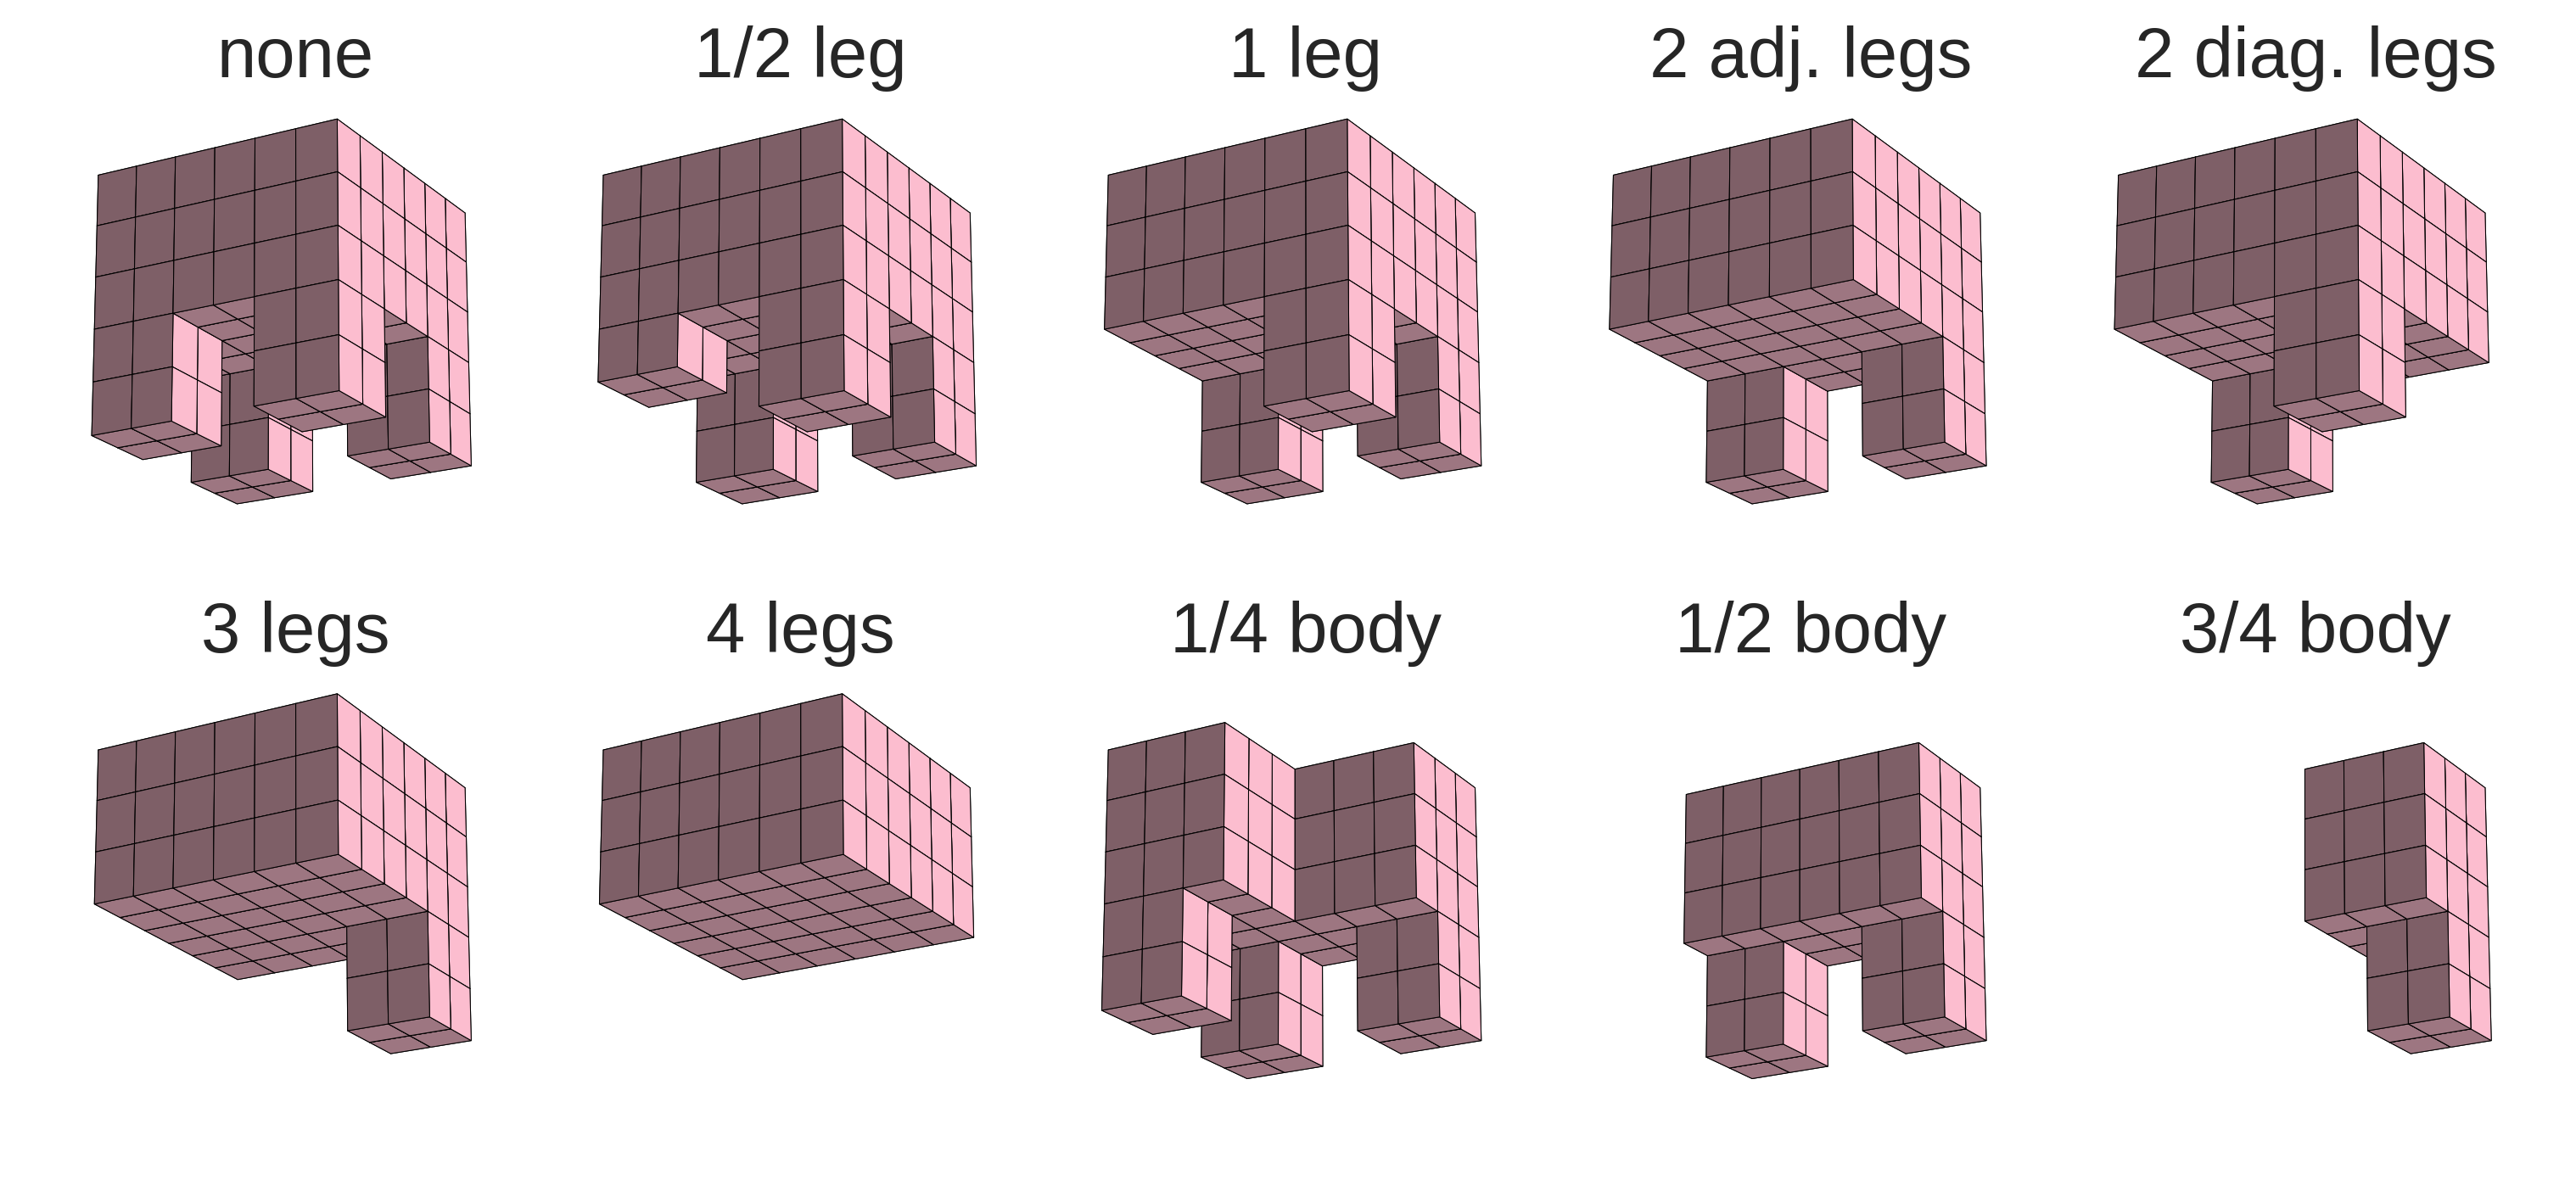
\includegraphics[trim={14pt 0 14pt 0},clip,width=0.9\linewidth]{Chapter05/fig/damage_scenarios.png}\\
% \vspace{-1em}
\caption{\label{fig5:scenarios}The various amputations applied in our experiments. 
The predamage robot (amputation = `none') is shown for reference.}
\vspace{-13pt}
\end{center}
\end{figure}


\subsection{The recovery options.}


Each damage scenario removes structure and breaks the robot's functionality: the robot loses voxels and its ability to walk.
We here consider two options for function recovery: 
\begin{enumerate}
    \setlength{\itemsep}{3pt}
    \item \textbf{Controller readaptation.}
    A new controller is optimized for locomotion with the damaged structure, as in \cite{bongard2006resilient,cully2015robots}.
    The only parameter subject to (re)optimization is the phase offset, $\phi_i$, of each voxel.
    \item \textbf{Shapeshifting.} The shape of the damaged structure is optimized for locomotion with the existing controller.
    The only parameter subject to optimization is the baseline rest length, $b_i$, of each voxel.
\end{enumerate}


\subsection{The shape change.}


The body is reshaped 
\textit{prior to} behavior (i.e., before the controller is turned on), analogous to a prenatal developmental stage.
This is done by adjusting the robot's shape, $\mathcal{S}$, as defined in Eq.~\ref{eq:shape}.
Then, behavior results from oscillations that are symmetrically distributed about this shape 
(Eq.~\ref{eq:beam_configuration}). 

The same kind of neural network that encodes controllers 
(i.e, a CPPN) 
was also used to encode 
the robot's shape.
However, the 
shape-encoding
networks output a rest beam length, $b_i$, between 0.25 and 2 cm (instead of a phase offset, $\phi_i$, between $-2\pi$ and $2\pi$).
Subject to the constraints outlined above,
optimization searches for shape-encoding networks that result in resting shapes that, when coupled with the original open-loop controller (previously optimized for the undamaged robot), synergize to recover forward movement.


\subsection{The optimization algorithm.}
\label{sec:optimization}


Shapes and control policies
are here optimized to displace the (simulated) robot in any direction using Age-Fitness-Pareto Optimization \citep{schmidt2011age}, 
an evolutionary algorithm that uses the concept of Pareto dominance and an objective of `age' (in addition to displacement) intended to promote diversity among candidate designs and prevent premature convergence.

 
A trial is initialized with a population of 50 randomly-generated designs with age zero.
Every generation, the population is first doubled by creating modified copies of each individual in the population (i.e., offspring, in which `age' is set equal to that of the parent), where modification occurs only to the encoding-network that is currently being optimized (either that of $\phi$ or $b$).
The age of each individual is then incremented by one. 
Next, an additional random individual (with age zero) is injected into the population (which now consists of 101 designs). 
Finally, selection reduces the population to its original size (50 designs) according to the two objectives of net displacement (maximized) and age (minimized): Starting with nondominated designs ($N=0$), successive Pareto fronts (containing designs dominated by exactly $N$ alternatives, for $N=1,2,\ldots$) are kept in their entirety until doing so would overfill the population past its original size; then, designs are selected one-by-one with probability proportional to their net displacement. (The 51 unselected designs are deleted.)


This process of random variation and directed selection is repeated for 
$G$ generations, in which
both the architectures and weights of the encoding networks are optimized:
Mutations add, modify or remove a particular vertex or edge.
Where modification of an edge reweights it (within -1 to 1 bounds) by adding a value randomly drawn from a normal distribution with mean zero and standard deviation 0.5.
Vertex modification swaps the node's activation function with a randomly chosen function in the set (adopted from \cite{kriegman2018interoceptive}): sin(), abs(), square(), sqrt(abs()); and the negations of those four. 




\begin{figure}[t]
    % \vspace{-1em}
    \centering
    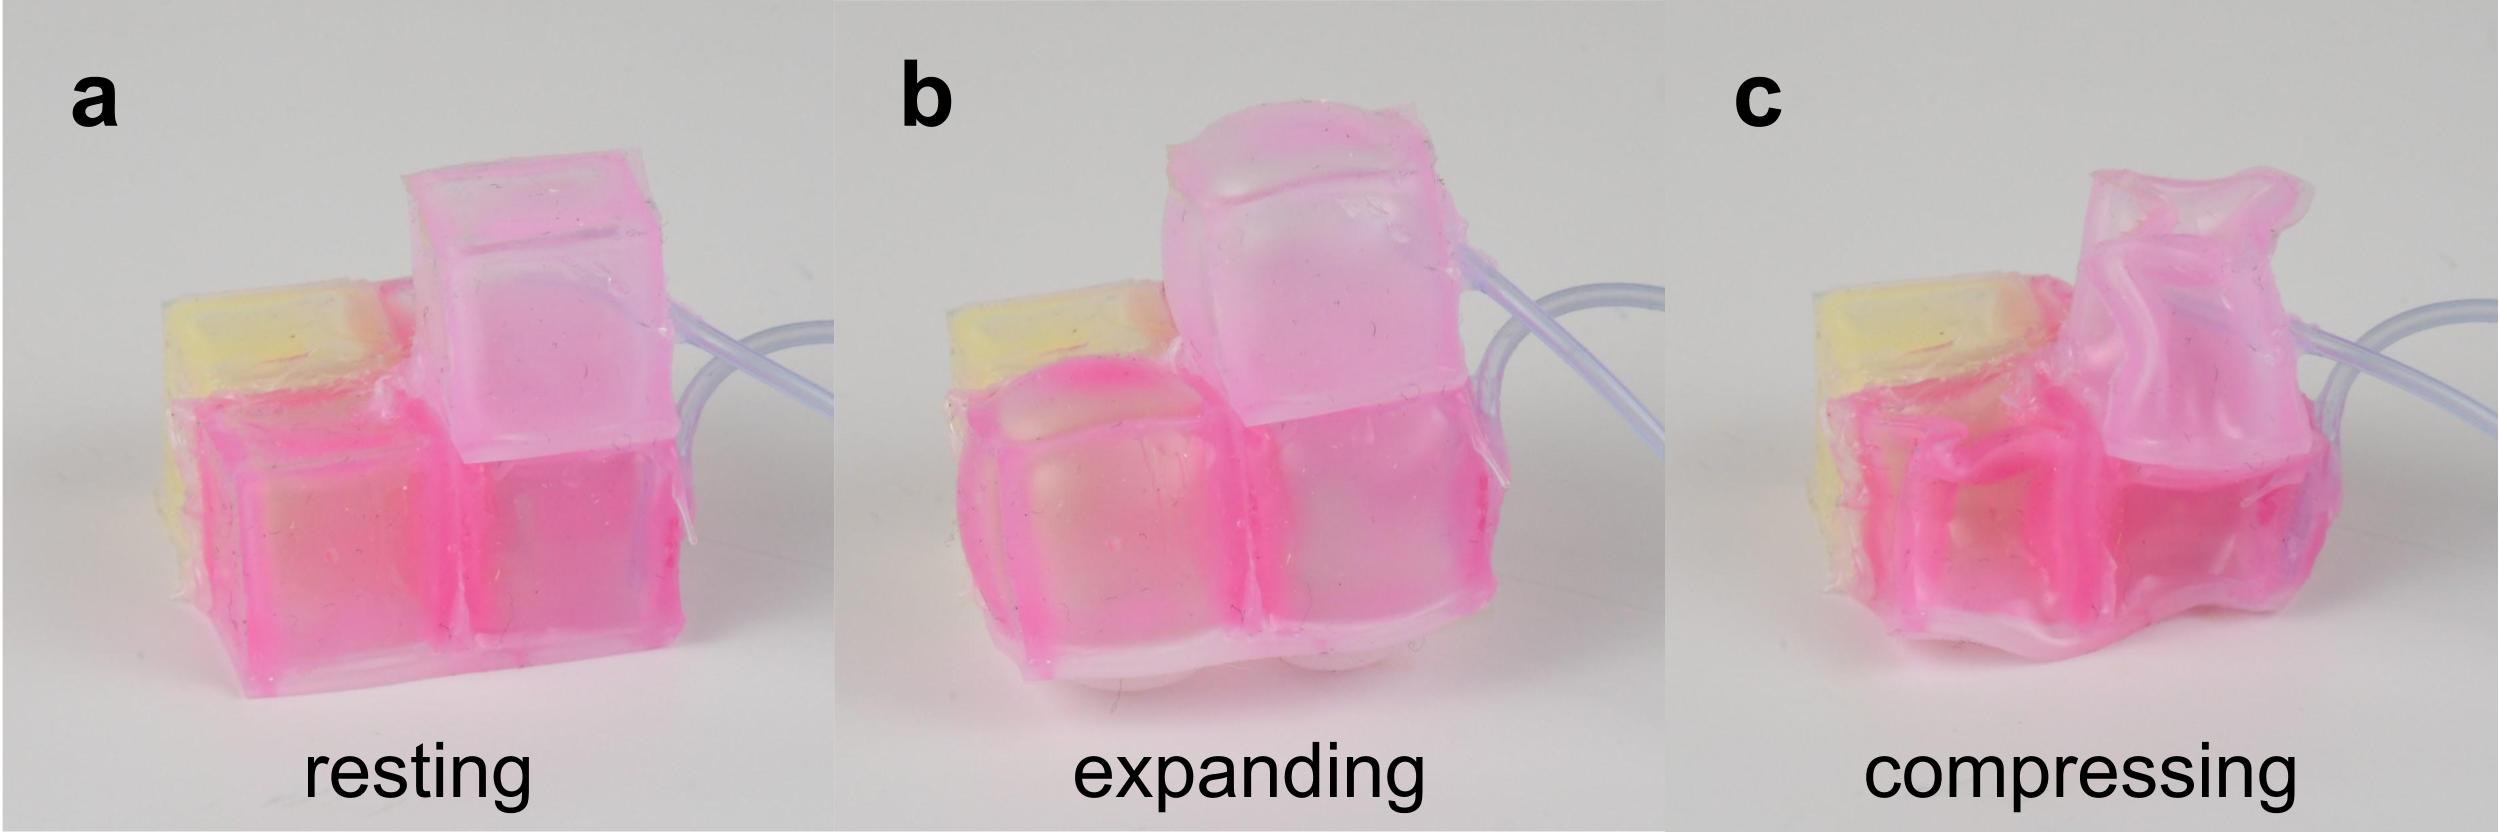
\includegraphics[width=0.7\linewidth]{Chapter02/fig/ExpansionContraction.jpg}
    % \vspace{-1.5em}
    \caption{A random morphology in the design space shown at atmospheric (resting; \textbf{a}), positive (expanding; \textbf{b}), and negative (compressing; \textbf{c}) pressure.}
    \label{fig:pressure}
\end{figure}





\subsection{The design space.}

Following \cite{hiller2011automatic} and \cite{kriegman2019automated}, our kit uses elastic voxels as building blocks of structure.
Here, we considered a \mbox{2-by-2-by-2} cartesian lattice workspace, within which voxels were connected together to form a robot.
At each x,y,z coordinate, voxels could either be passive, volumetrically actuated, or absent, yielding a total of $3^8=6561$ different configurations. 
We evaluated each configuration in simulation.



\begin{figure}[t]
    \centering
    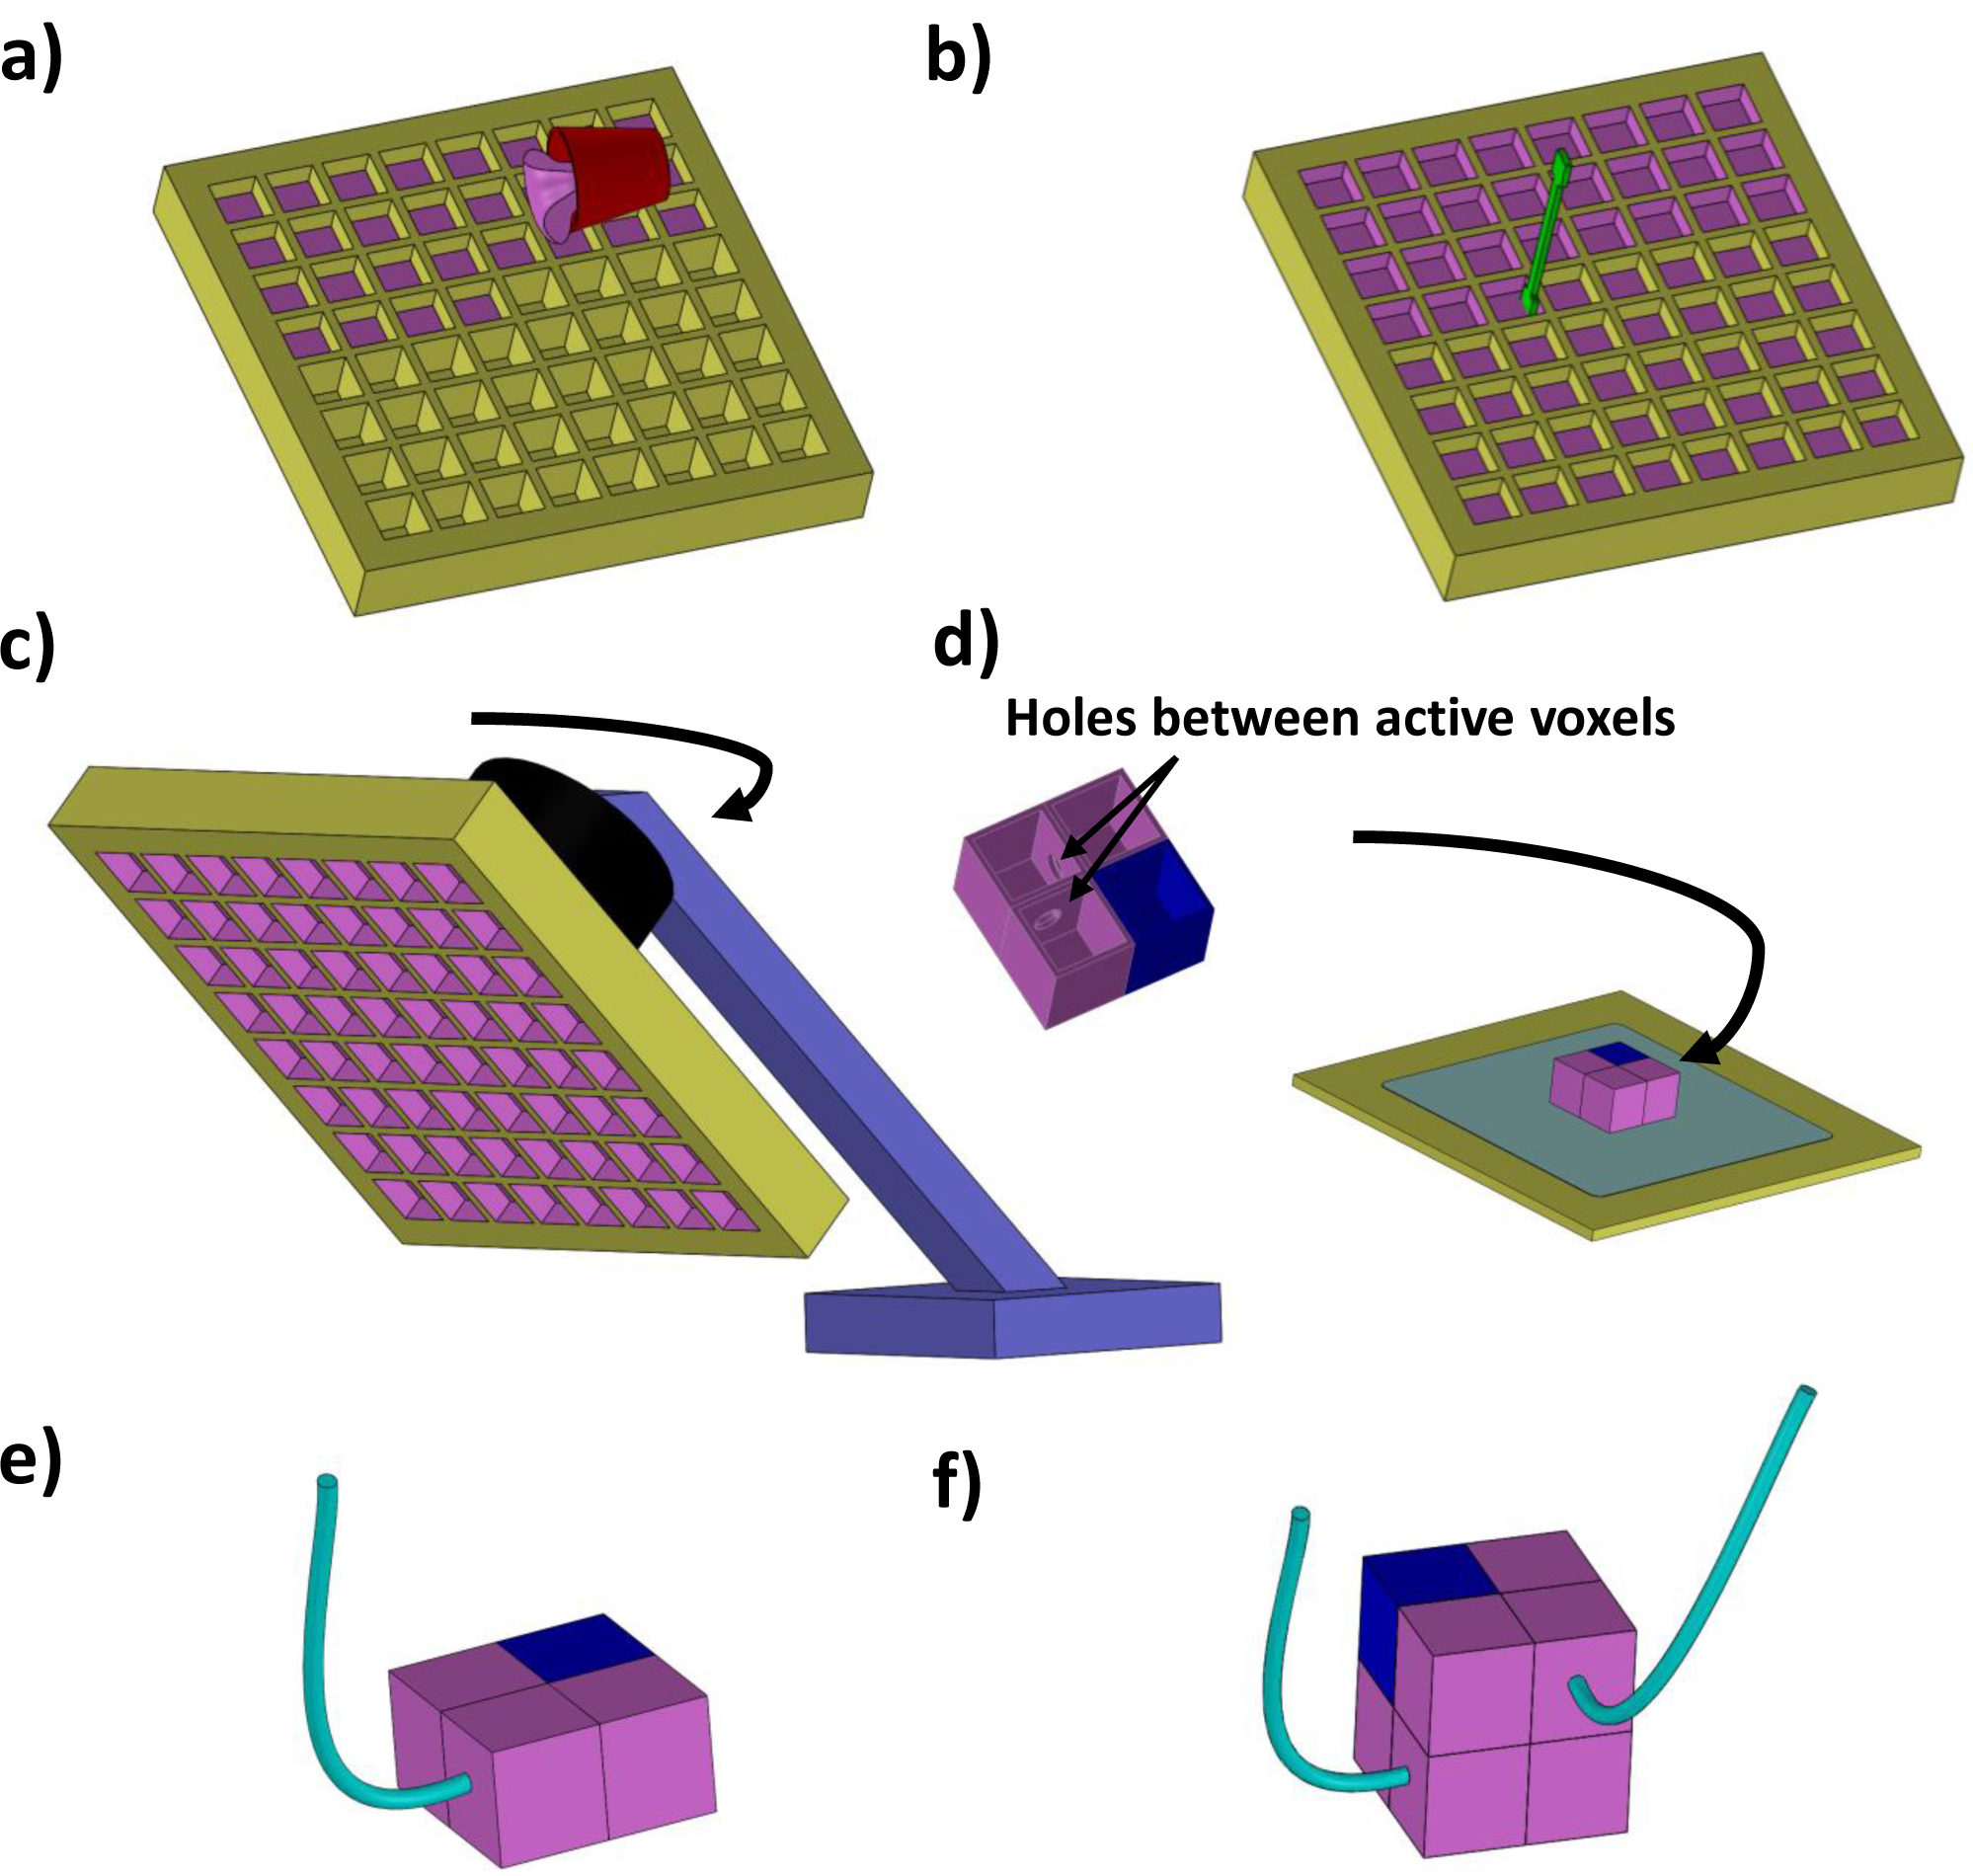
\includegraphics[width=0.7\linewidth]{Chapter02/fig/voxel_manufacturing.jpg}
    % \vspace{0pt}
    \caption{\textbf{Manufacturing modular soft robots.}
    Hollow, silicone voxels were created by partially filling an open-face mold with silicone (\textbf{a}), 
    using a spatula to spread it along the interior walls (\textbf{b}), and then securing the mold to a 1-axis rotational molding machine (\textbf{c}). This process allowed excess silicone to drip out of the mold, while spreading the remaining silicone into a thin uniform layer.
    The cured, bottomless voxels were then appropriately arranged and connected for each x,y slice of the design, and bonded with a shared bottom layer (\textbf{d}).
    Finally, tubing was attached (\textbf{e}), and the slices were stacked and bonded to form the design (\textbf{f}). 
    Video:
\href{https://youtu.be/jbQ2T7jIYRU}{\color{blue}\tt\textbf{youtu.be/jbQ2T7jIYRU}}.
    }
    \label{fig:real}
    % \vspace{-1.5em}
\end{figure}


\subsection*{The simulation.}

We used the soft-body physics engine Voxelyze \cite{hiller2014dynamic} to simulate robots composed of actuating and/or passive, elastic voxels.
The simulator models the distance between adjacent voxels as Euler-Bernoulli beams (critically damped; $\zeta=1$).
Additionally, a collision detection system monitors the distance between the voxels on the surface of the robot at each timestep.
If a pair of surface voxels are detected to collide (intersect), a temporary beam (underdamped; $\zeta=0.8$) is constructed between the two until the collision is resolved. 
% (This temporary bond is deleted once the voxels no longer intersect.)

Designs were simulated with a gravitational acceleration of -9.81 m/s$^2$, and initialized on top of an infinite surface plane at $z=0$.
Coulomb friction is applied to voxels in contact with the surface plane.
% Slow (global?) damping coefficient of 0.01 was used.
Voxels were simulated to have 1 cm$^3$ resting volume (resting beam lengths), with Young's modulus $10^7$ Pa, Poisson's ratio 0.35, 
% density $10^6$ kg/m$^3$, % todo: this cannot be right
and coefficients of static and kinetic friction of 1 and 0.5, respectively.
These hyperparameters were adopted from \cite{kriegman2019automated}.
For more details about how the physics are actually modeled, see \cite{hiller2014dynamic}.

Volumetric actuation was implemented by varying the rest length between voxels, in all three dimensions, when computing the elastic force between them.
Volumetric expansion in simulation and reality are both roughly spherical
(Fig.~\ref{fig:pressure}b), but compression in reality is more complex
and difficult to simulate: 
the voxels buckle (Fig.~\ref{fig:pressure}c).
So volumetric actuation was here limited to expansion only ($+90\%$ rest volume).
The active voxels expand in phase with each other 
as dictated by
a central pattern generator:
a sine wave with frequency 4 Hz and amplitude 1.9 cm$^3$.
When the sine wave is at or below zero, the active voxels remain at their resting volume (1 cm$^3$).
This produced quasistatic dynamics.

Each design was simulated for 8831 timesteps, with a stepsize of 0.000453 seconds, resulting in a total simulation time of 4 seconds.
During the first 552 times steps (0.25 sec), the design was allowed to settle under gravity before actuation begins, ensuring that movement (if any) is a result of actuation, rather than passively falling forward.
Just before actuation, the design's initial center of mass is recorded as $(x_0, y_0, z_0)$.
The active voxels are then actuated for 3.75 sec at 4 Hz, or 15 actuation cycles.

An exhaustive search of all 6561 designs (in batches of 50) took 58 CPU hours (1.8 wall-clock hours) on a single AMD Ryzen threadripper 1950X 16-core/32-thread processor.
Fitness was taken to be the net displacement (away from the origin in any direction) of the design's center of mass, in terms of euclidean distance in the plane,
where the origin is defined by the $x,y$ components of the design's initial center of mass $(x_0, y_0)$.
Fitness is thus defined as:
\begin{equation}
    \label{eq:fitness}
    F=\sqrt{(x_t-x_0)^2+(y_t-y_0)^2} \,,
\end{equation}
where $x_t,y_t$ are the final coordinates of the design at the end of the evaluation period.



\subsection{Reality.}


Following \citet{kriegman2019automated}, simulated voxels were realized physically as pneumatically-actuated, hollow silicone voxels.
The physical robot in \cite{kriegman2019automated} was constructed to transfer symmetrical shape change, so its actuated voxels were distributed symmetrically and hooked into a single pressure inlet.
Thus, pressure oscillations occurred symmetrically in phase, and the robot could only pulse in place.
Moreover, due to thin voxel walls relative to overall voxel size, and the tubing and glue used to bond them together, the robot in \cite{kriegman2019automated} could not fully support its own weight.
The robot was lifted off the ground by placing it on top of a small petri dish, positioned underneath a segment of entirely passive voxels in the center of the robot's ventral surface.
This permitted ventral (and more extreme global) changes in surface curvature, yielding successful sim2real transfer of shape change, 
but not locomotion.


The construction kit presented here rectifies the weight issue by miniaturizing the voxels|voxel length was halved (from 3cm to 1.5cm) and the wall thickness remained the same (1mm), reducing voxel mass from 4.3g to 1.2g (including tubing but not pneumatic connectors).
Further, the inter-voxel tubing and glue was replaced with holes punched through the walls of adjacent active voxels in the same x,y slice, before attaching them with a shared bottom layer (Fig.~\ref{fig:real}d).
Finally, locomotion is now possible because separate contiguous sections of voxels in each slice can be arbitrarily actuated in or out of phase with other sections across the body.


\subsection{The build protocol.}


The voxels were manufactured using a single-axis rotational molding machine.
First, an open-face mold was fabricated by interlacing 26 acrylic strips into a flat base, to form a lattice of cubic concavities, resembling an ice-cube tray (Fig.~\ref{fig:real}a). Mold components were laser-cut (VLS2.30, Universal Laser System) from a flat acrylic sheet with a thickness of 0.025 inch.
Next, silicone (Dragon Skin 10 Fast; Smooth-On, Inc.) was poured into the acrylic mold (Fig.~\ref{fig:real}a), and a spatula was used to spread the silicone along the interior walls of each cavity (Fig.~\ref{fig:real}b). Colored pigment was added to each batch of silicone to indicate whether the voxel was active or passive, simplifying the assembly process. Here we used pink for active voxels and blue or yellow for passive voxels.

The mold was then flipped upside down and secured to a 1-axis rotational molding machine. The machine was clamped to a table with binder clips, angled $45^{\circ}$ relative to horizontal, and set to rotate $90^{\circ}$ every 45 seconds (Fig.~\ref{fig:real}c).
This allowed the silicone to flow and evenly coat the walls of the mold, as excess silicone dripped out. 
After the voxels partially cured for 25 minutes at room temperature, the mold was moved to an incubator, with a temperature of $60^{\circ}$C for another 20 minutes. 
(Without an incubator, the silicone will take 75 minutes to fully cure at room temperature.)

The above steps were then repeated to add an additional layer of silicone.
Once the second layer cured, the bottomless voxels were removed from the mold using an X-Acto knife, and excess silicone around their edges was trimmed.

In the next step, each x,y slice (or dorsal plane) of the design was assembled by using Sil-Poxy (Smooth-On, Inc.) to bond adjacent voxels and prevent the slice from shifting.
Holes were then punched between adjacent active voxels so that contiguous collections of voxels could be actuated together in phase.
Each actuator group needed to contain at least one voxel on the surface of the design so that it could be controlled by an external pressure inlet.
To create the bottom layer, two 1mm-thick rulers were attached to an acrylic substrate using double-sided tape and silicone was poured in the space between them. 
Then, the slice of bottomless voxels was flipped, open-side down, onto this uncured silicone layer (Fig.~\ref{fig:real}d). 

After the bottom layer cured, a thin layer of silicone was applied with a popsicle stick along the outermost portions of the interstices of the voxels, bonding adjacent voxels (without gluing over inter-voxel holes).
Then, the slice was cut from the silicone sheet and a hole was poked into the side of one exterior voxel from each group of active voxels.
Next, a 1/32'' ID silicone tube was inserted into the hole, and glued in place with Sil-Poxy, applied with a Q-tip (Fig.~\ref{fig:real}e). 
The end of this tube was then connected to a straight pneumatic connector, which was connected to 1/16'' ID silicone tubing.

Occasional imperfections in alignment, silicone thickness, or inter-voxel hole sizes would result in leaky structures. 
Leaks were detected by filling a beaker with water, submerging the voxels, and inflating them. 
Bubbles would emanate from leaks, which were repaired with Sil-Poxy.
After repairing any leaks, the slices were stacked on top of each other and bonded together using a thin layer of silicone (Fig.~\ref{fig:real}e). 
Finally, these layers were connected pneumatically with assorted pneumatic connectors, attached to 1/16'' ID silicone tubes. 



\section{Results}
\label{sec:results}


\begin{wrapfigure}{r}{0.475\linewidth}
\vspace{-14pt}
\centering
\includegraphics[width=0.8\linewidth]{Chapter02/fig/legend.pdf}
% \vspace{-15pt}
\caption{The 2D tessellation of 8D ternary vector space used in Fig.~\ref{fig:sim}.}
\label{fig:tesselation}
\vspace{-1em}
\end{wrapfigure}


To test the effects of morphology on fitness and sim2real transfer success, it is useful to first visualize the design space. 
However, because there are eight cartesian voxel coordinates in the chosen workspace, the design space here is eight dimensional, which is difficult to draw (let alone conceptualize) without dimensionality reduction.
By nesting the dimensions of a search space onto a single plot (Fig.~\ref{fig:tesselation}), the entire space can be visualized as a 2D heatmap.
This strategy was used by \citet{cully2015robots} to neatly visualize the predicted fitness of a very large library of control policies, as a function of the time a robot's six limbs were in contact with the simulated ground plane: 6D quinary control space was mapped to 2D, by nesting pairs of dimensions within each other.



\begin{figure}[t]
    % \vspace{-2em}
    \centering
    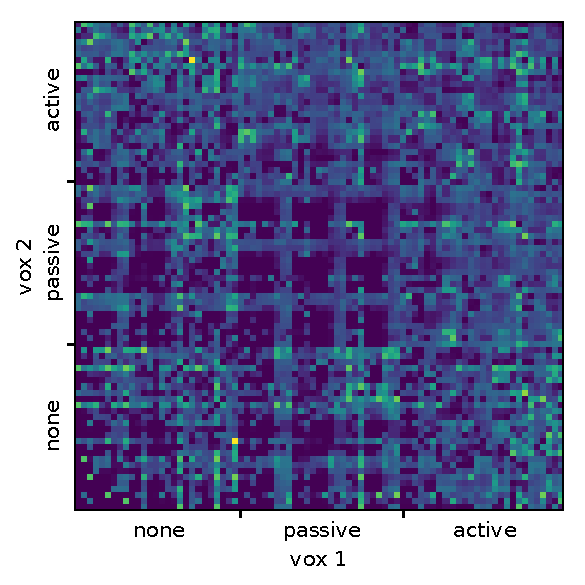
\includegraphics[width=0.7\linewidth]{Chapter02/fig/design_space.pdf}
    % \vspace{-2em}
    \caption{\textbf{Simulating modular soft robots.}
    The design space is plotted as a heatmap, containing one cell for each of the 6561 possible configurations.
    Lighter colored cells are fitter designs (Eq.~\ref{eq:fitness}).
    Each design is defined by a vector of eight ternary values, indicating what kind of voxel (none, passive, or active) the design contains at the eight lattice points in the $2\times2\times2$ workspace.
    The 8D ternary vector is reduced to a 2D heatmap by nesting pairs of dimensions within each other: four, nested $3\times3$ grids result in a $3^4\times3^4=81\times81$ overall heatmap.
    }
    \label{fig:sim}
    % \vspace{-1em}
\end{figure}



Here, the 8D ternary morphology space was reduced to 2D by plotting pairs of dimensions nested within each other (Fig.~\ref{fig:sim}).
The pixel in the exact center of Fig.~\ref{fig:sim}, for instance, represents the configuration consisting entirely of passive voxels, and thus cannot locomote ($F=0$).
Likewise, the pixel in the top right-hand corner of the heatmap represents the configuration of all active voxels (Fig.~\ref{fig:transfer}d), which actuated symmetrically in phase, and thus (given its flat ventral surface) could not locomote across the flat ground plane ($F=0$).
Finally, the pixel in the bottom left-hand corner contains no voxels at all, and thus $F=0$.


For locomotion, a good design obviously needs to have a body, rather than none at all.
With open-loop, in-phase actuation, designs also need to have asymmetrical mass and/or actuator distributions, or they will not generate any forward movement.
However it is not clear, even for this minimal design space, exactly which asymmetrical designs will yield the highest fitness.
Yet we can see small clusters and lines of similarly colored pixels in Fig.~\ref{fig:sim}, representing morphologically similar designs with similar fitness.
This suggests that these configurations and substructures would be relatively stable under random mutations or errors in fabrication.


Because fitness was measured by displacement in any direction away from the origin (Eq.~\ref{eq:fitness}), there are four configurations---rotations, in the x,y plane, of a single geometry and distribution of passive and active voxels---with different behaviors (they moved in different directions) but very similar (if not identical) fitness.
There were also some configurations that, when rotated upward (in the x,z or y,z plane) fell into the same basic orientation and behavior but with a slightly different heading.
Thus, configurations with similar fitness (similarly colored pixels) are reflected across multiple, nested planes of symmetry in Fig.~\ref{fig:sim}.
These symmetries can also be seen in the manufactured robots (Fig.~\ref{fig:teaser}b).
The uniqueness of designs (i.e., the size of the search space of morphologies) is therefore a function of how behavior is measured.



\begin{figure*}[t]
    \centering
    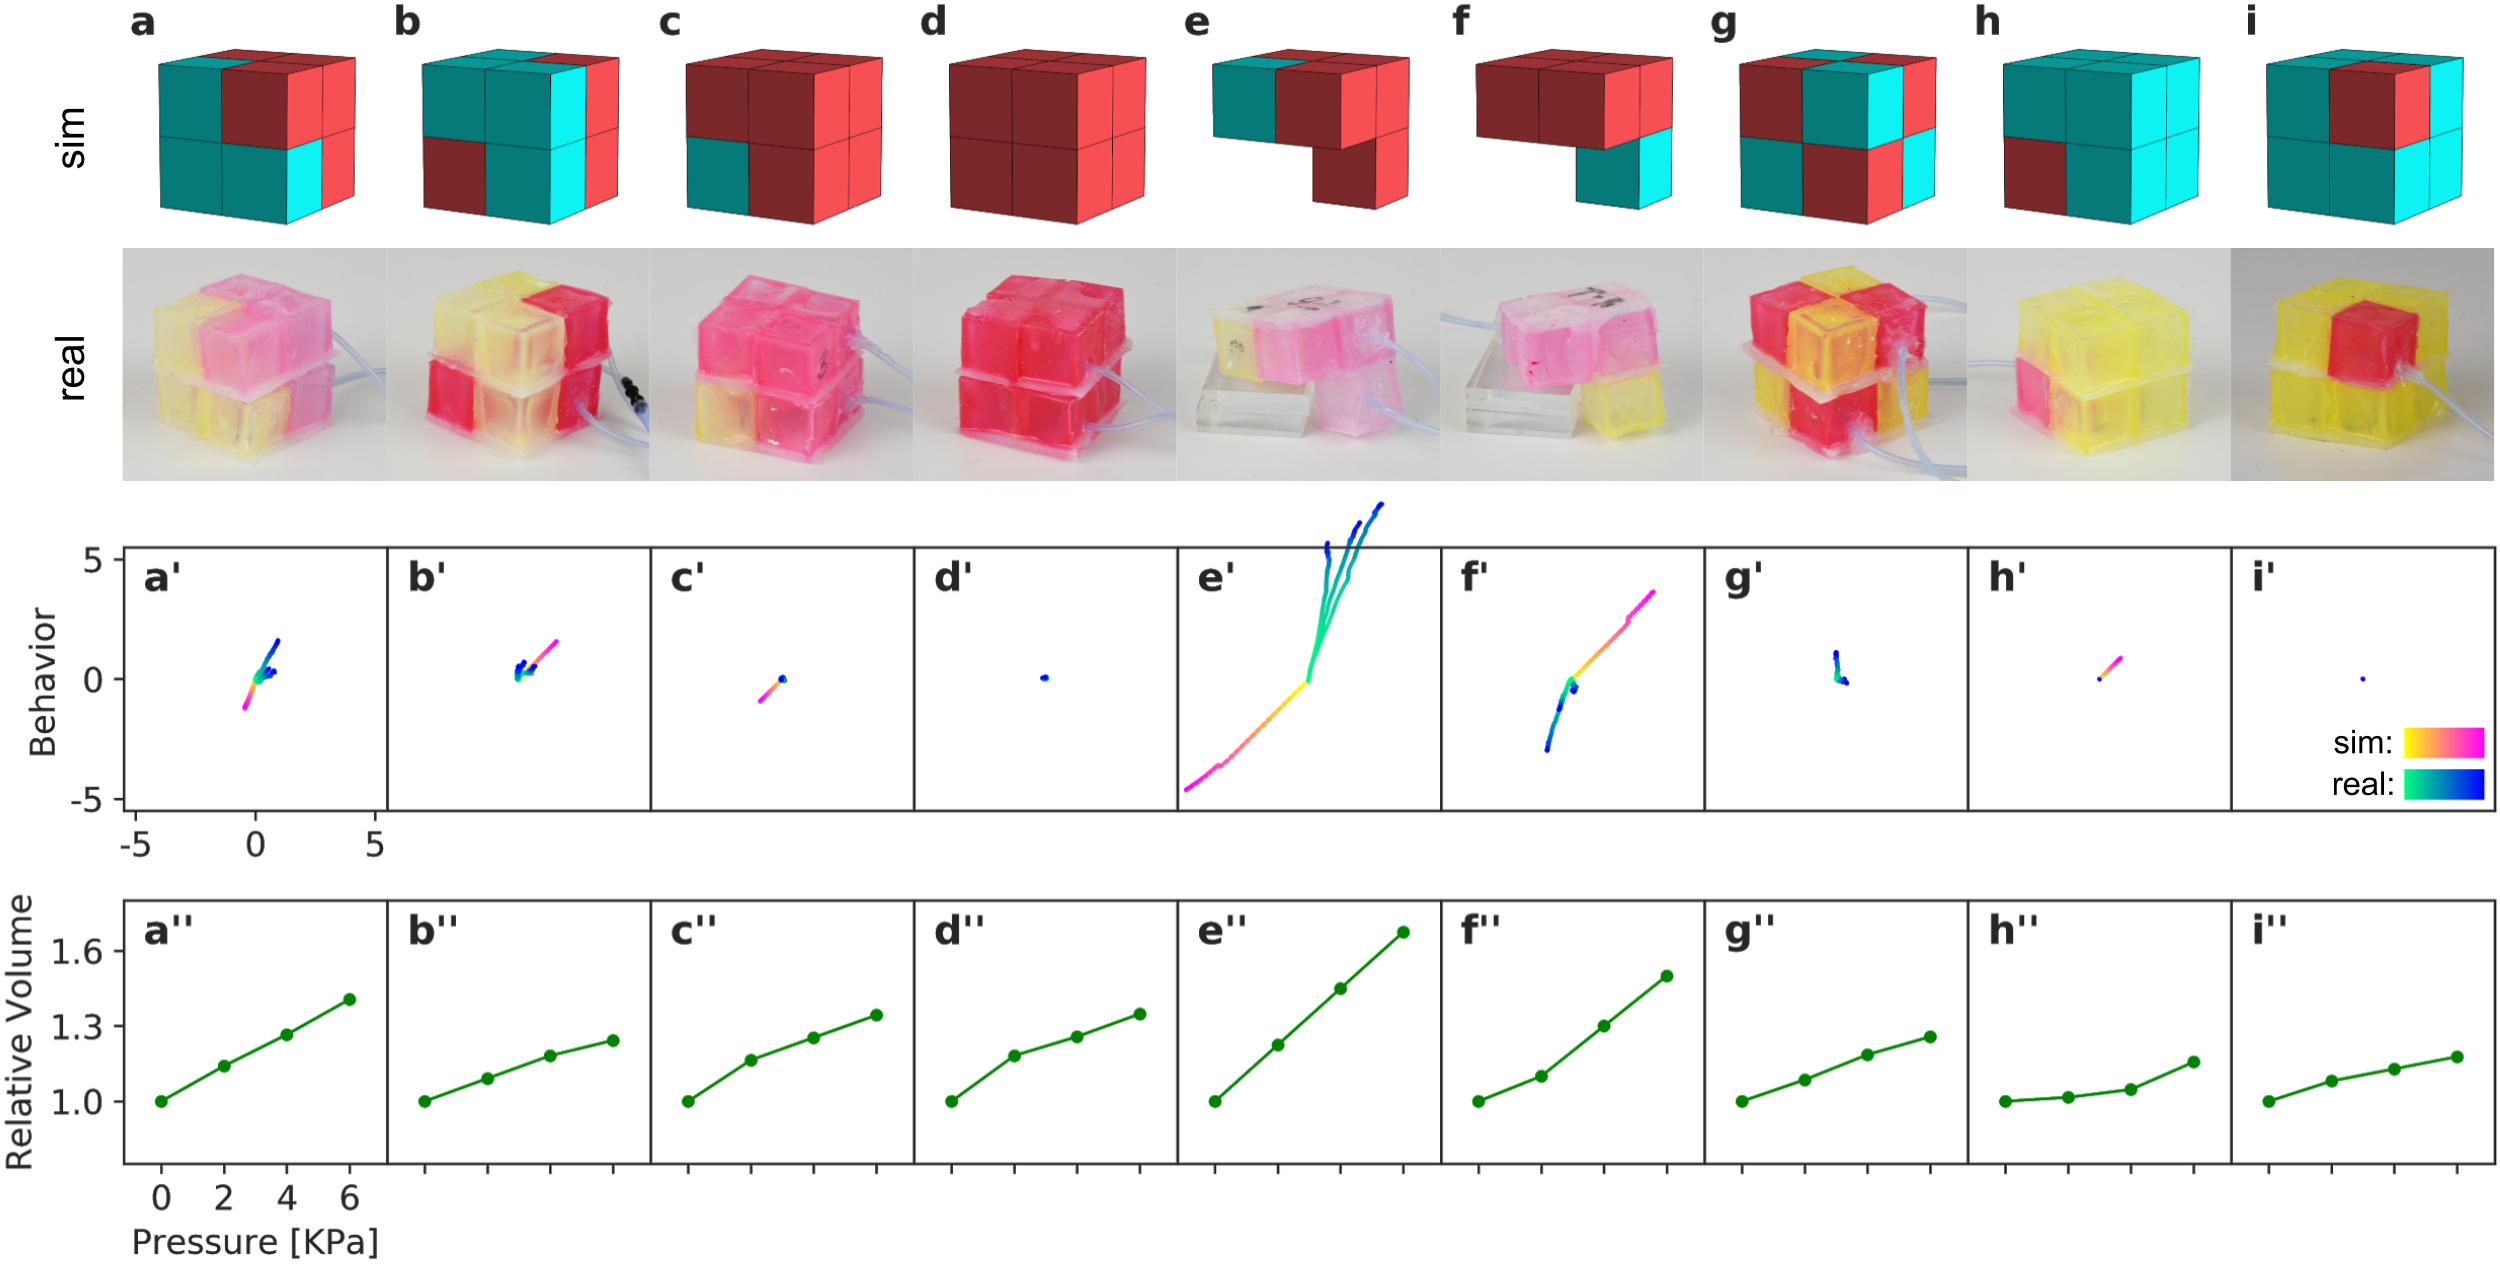
\includegraphics[width=\linewidth]{Chapter02/fig/YaleTraces2.png}
    % \vspace{-1.75em}
    \caption{\textbf{Measuring transferal from simulation to reality}.
    Nine designs (\textbf{a-i}) were evaluated three times each in reality (green-to-blue gradient colored curves in \textbf{a\textquotesingle-i\textquotesingle}).
    The behavioral trajectories start at the origin (green) and end at the robot's final XY destination (blue) (in centimeters).
    The simulated movement tracks (yellow-to-pink curves) are superimposed on top of the real ones.
    The relative volume (normalized by rest volume) was also recorded for each design at four points during actuation under water (\textbf{a\textquotesingle\textquotesingle-i\textquotesingle\textquotesingle}).
    % The two designs that displaced farthest in the plane (e and f) also achieved the largest volumetric expansion.
    The simulated and real behavior of designs e and f can be observed here:
    \href{https://youtu.be/UqjvmkYa9u4}{\color{blue}\tt\textbf{youtu.be/UqjvmkYa9u4}}.
    }
    \label{fig:transfer}
    % \vspace{-1.25em}
\end{figure*}
 

\begin{figure}[t]
    \centering
    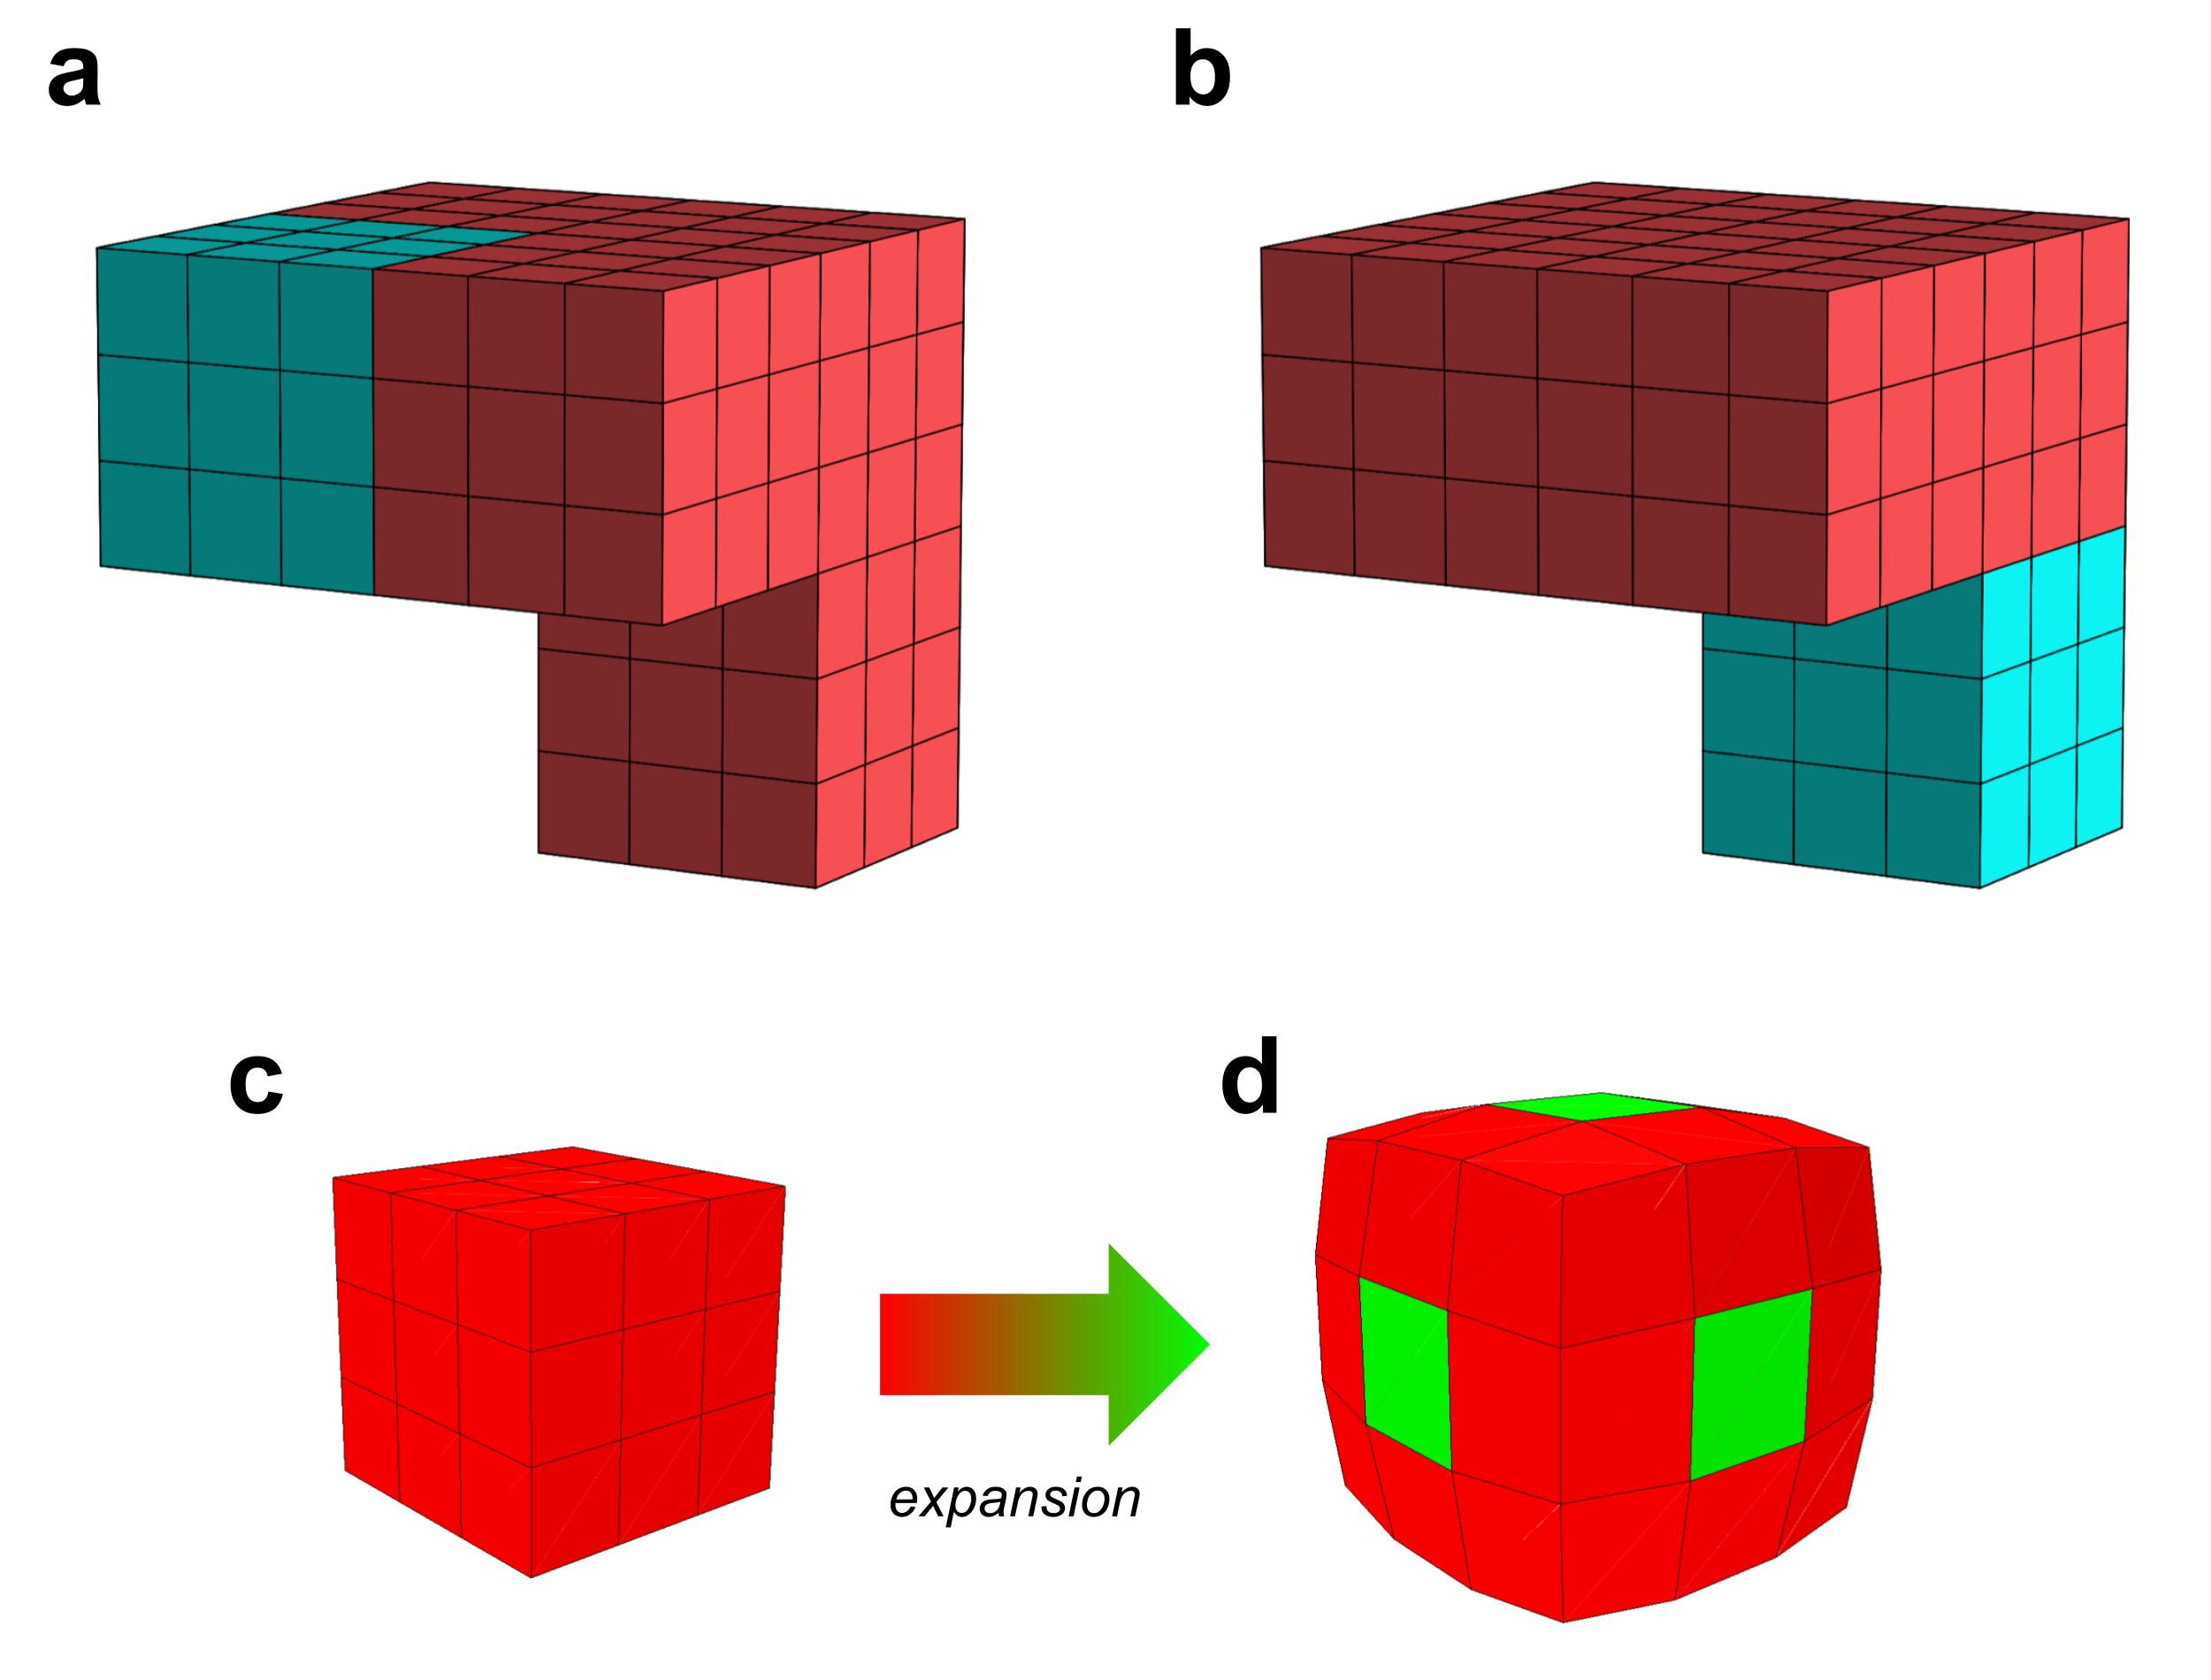
\includegraphics[width=0.65\linewidth]{Chapter02/fig/Yale_High_Res_Sim.jpg}
    % \vspace{-1em}
    \caption{A higher resolution model in which each silicone voxel is approximated by a 3-by-3-by-3 group of simulated subvoxels: a high-res voxel.
    The design in \textbf{a} and \textbf{b} are high-res instantiations of those in Figs.~\ref{fig:transfer}e and \ref{fig:transfer}f, respectively. 
    Spherical volumetric expansion in a high-res voxel (\textbf{c}) was approximated by increasing the rest length between the centermost subvoxel and the subvoxels at center of each face (green subvoxels in \textbf{d}).
    }
    \label{fig:hi_res_sim}
    % \vspace{-1.25em}
\end{figure}



Fig.~\ref{fig:transfer} shows the behavior of nine different designs in simulation and reality.
The real robot was actuated 90 times at 6 kPa pressure on a surface covered with cornstarch 
(Argo\textregistered, ACH Food Companies, Inc.) 
to reduce friction, and is compared to 23 simulated actuation cycles.
Seven of the nine designs filled the cubic workspace with passive and active voxels, while the other two share a more complex geometry: a single-voxel limb attached to the face of a 2-by-2 plane of voxels (Fig.~\ref{fig:transfer}e,f).
In one, the limb is active (Fig.~\ref{fig:transfer}e), in the other it is passive (Fig.~\ref{fig:transfer}f).
These two designs achieved the two highest fitness scores (Eq.~\ref{eq:fitness}), in both simulation and reality.

By this measure, the reality gap appears small.
However, these simulated designs move very differently from their manufactured equivalents.
The simulated morphology in Fig.~\ref{fig:transfer}e pushes off its active limb, whereas in reality the design uses its limb to pull itself forward, in the opposite direction.
Likewise, the simulated morphology in Fig.~\ref{fig:transfer}f pushes off its active 2-by-2 torso, whereas in reality the design uses its torso to pull itself forward, in the opposite direction.

\citet{majidi2013influence} showed that the interfacial shear strength and coefficient of friction of the surface on which their soft robot undulated determined the direction of locomotion. They decomposed friction into load- and area controlled terms for point and surface contacts, respectively. 
On slippery surfaces with low interfacial shear resistance, the robot anchored about the point contact (expanded section) for locomotion and pulled its surface contact (passive segment). However, on surfaces with high interfacial shear resistance, the robot anchored about the surface contact and pulled the point contact toward it. 
We hypothesize that such differences in tribological properties could have caused our designs to move in opposite directions in simulation and reality.

In an attempt to test this hypothesis and reduce the simulation-reality discrepancies that cause the virtual configurations in Fig.~\ref{fig:transfer} to move differently than their physical realizations, we performed a grid search of various simulation hyperparameters, including the coefficients of static and kinetic friction.
However, we could not identify a pair of friction coefficients that resulted in correct movement heading for all nine of the behaving designs (Fig.~\ref{fig:transfer}a\textquotesingle-i\textquotesingle).
This could be due to either low precision or low accuracy of the model.
To isolate and test the former possibility, we increased the resolution of the simulated surface contact geometry by modeling each silicone voxel as a 3-by-3-by-3 group of simulated ``subvoxels'' (Fig.~\ref{fig:hi_res_sim}),
and then re-ran the parameter sweep.
Still, we could not find friction settings in which the simulated movement direction matched the ground truth across all designs simultaneously.
This suggests that the accuracy of Coulomb friction model may be insufficient to model this type of movement.

The Coulomb approximation assumes that friction is simply proportional to the vertical component $N$ of the reaction force, and independent of the contact area. 
However, friction is also a function of the surface area and interfacial shear strength $\tau$, a fixed constant which is mostly governed by adhesion or mechanical interlocking between the contacting surfaces. 
A better model would thus consider friction as a function of both the normal force and the interfacial shear strength.
However, before fundamentally changing the simulator,
we plan to evaluate designs in noisy environments with imperfect control over actuation characteristics to avoid ascribing high fitness to designs that exploited unrealistic properties of the simulation \cite{jakobi1995noise}.
Additionally, data from reality could be used to automatically tune  the geometry and resolution of the simulated finite elements \cite{bongard2006resilient}, or to predict the kinds of behaviors that are more likely to successfully transfer \cite{koos2012transferability}, and which should be tested next \cite{bongard2006resilient}. 
Concurrently, we are investigating additional physical surfaces with varied tribological properties in an attempt to match reality to simulation.



% The best design achieved the largest volumetric expansion (Fig.~\ref{fig:transfer}a\textquotesingle\textquotesingle)...





% 
\begin{figure}[t]
    % \vspace{-2em}
    \centering
    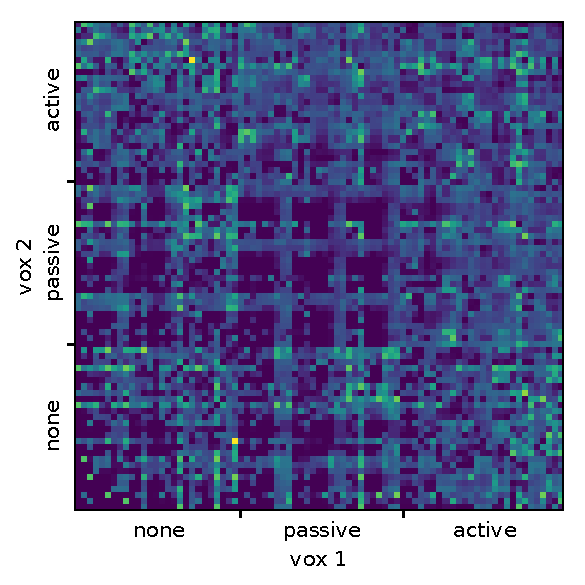
\includegraphics[width=0.7\linewidth]{Chapter02/fig/design_space.pdf}
    % \vspace{-2em}
    \caption{\textbf{Simulating modular soft robots.}
    The design space is plotted as a heatmap, containing one cell for each of the 6561 possible configurations.
    Lighter colored cells are fitter designs (Eq.~\ref{eq:fitness}).
    Each design is defined by a vector of eight ternary values, indicating what kind of voxel (none, passive, or active) the design contains at the eight lattice points in the $2\times2\times2$ workspace.
    The 8D ternary vector is reduced to a 2D heatmap by nesting pairs of dimensions within each other: four, nested $3\times3$ grids result in a $3^4\times3^4=81\times81$ overall heatmap.
    }
    \label{fig:sim}
    % \vspace{-1em}
\end{figure}
  % moved inside 3_results.tex
% 
\begin{figure*}[t]
    \centering
    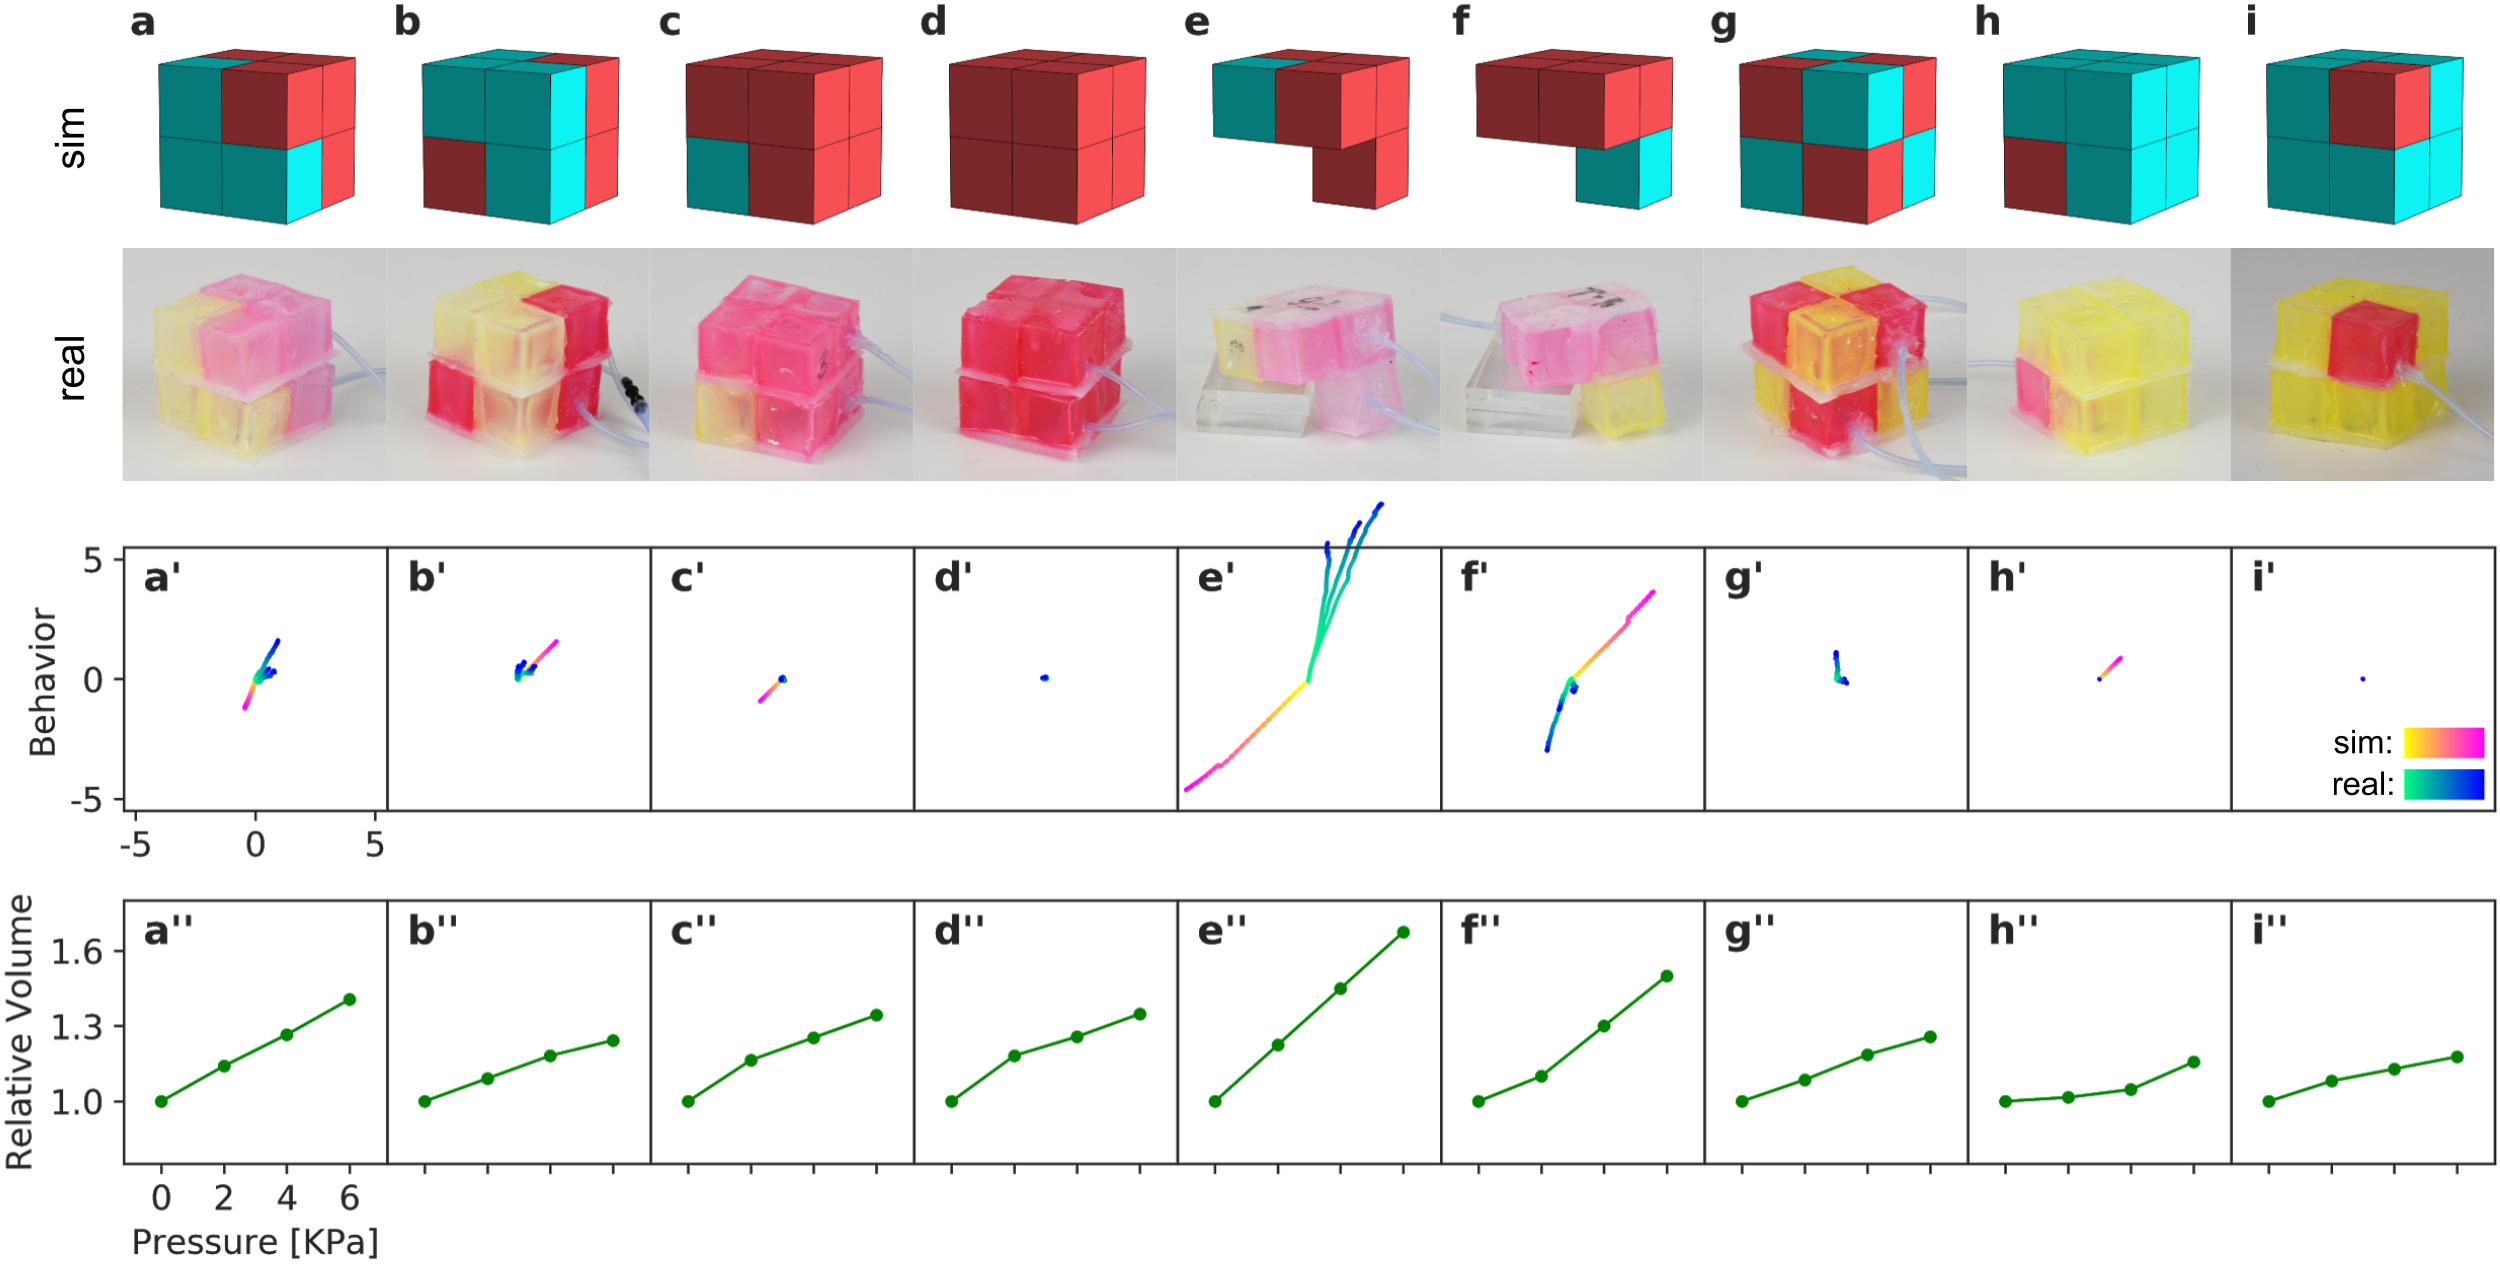
\includegraphics[width=\linewidth]{Chapter02/fig/YaleTraces2.png}
    % \vspace{-1.75em}
    \caption{\textbf{Measuring transferal from simulation to reality}.
    Nine designs (\textbf{a-i}) were evaluated three times each in reality (green-to-blue gradient colored curves in \textbf{a\textquotesingle-i\textquotesingle}).
    The behavioral trajectories start at the origin (green) and end at the robot's final XY destination (blue) (in centimeters).
    The simulated movement tracks (yellow-to-pink curves) are superimposed on top of the real ones.
    The relative volume (normalized by rest volume) was also recorded for each design at four points during actuation under water (\textbf{a\textquotesingle\textquotesingle-i\textquotesingle\textquotesingle}).
    % The two designs that displaced farthest in the plane (e and f) also achieved the largest volumetric expansion.
    The simulated and real behavior of designs e and f can be observed here:
    \href{https://youtu.be/UqjvmkYa9u4}{\color{blue}\tt\textbf{youtu.be/UqjvmkYa9u4}}.
    }
    \label{fig:transfer}
    % \vspace{-1.25em}
\end{figure*}
 % also moved inside results for positioning

\begin{figure}[t]
    \centering
    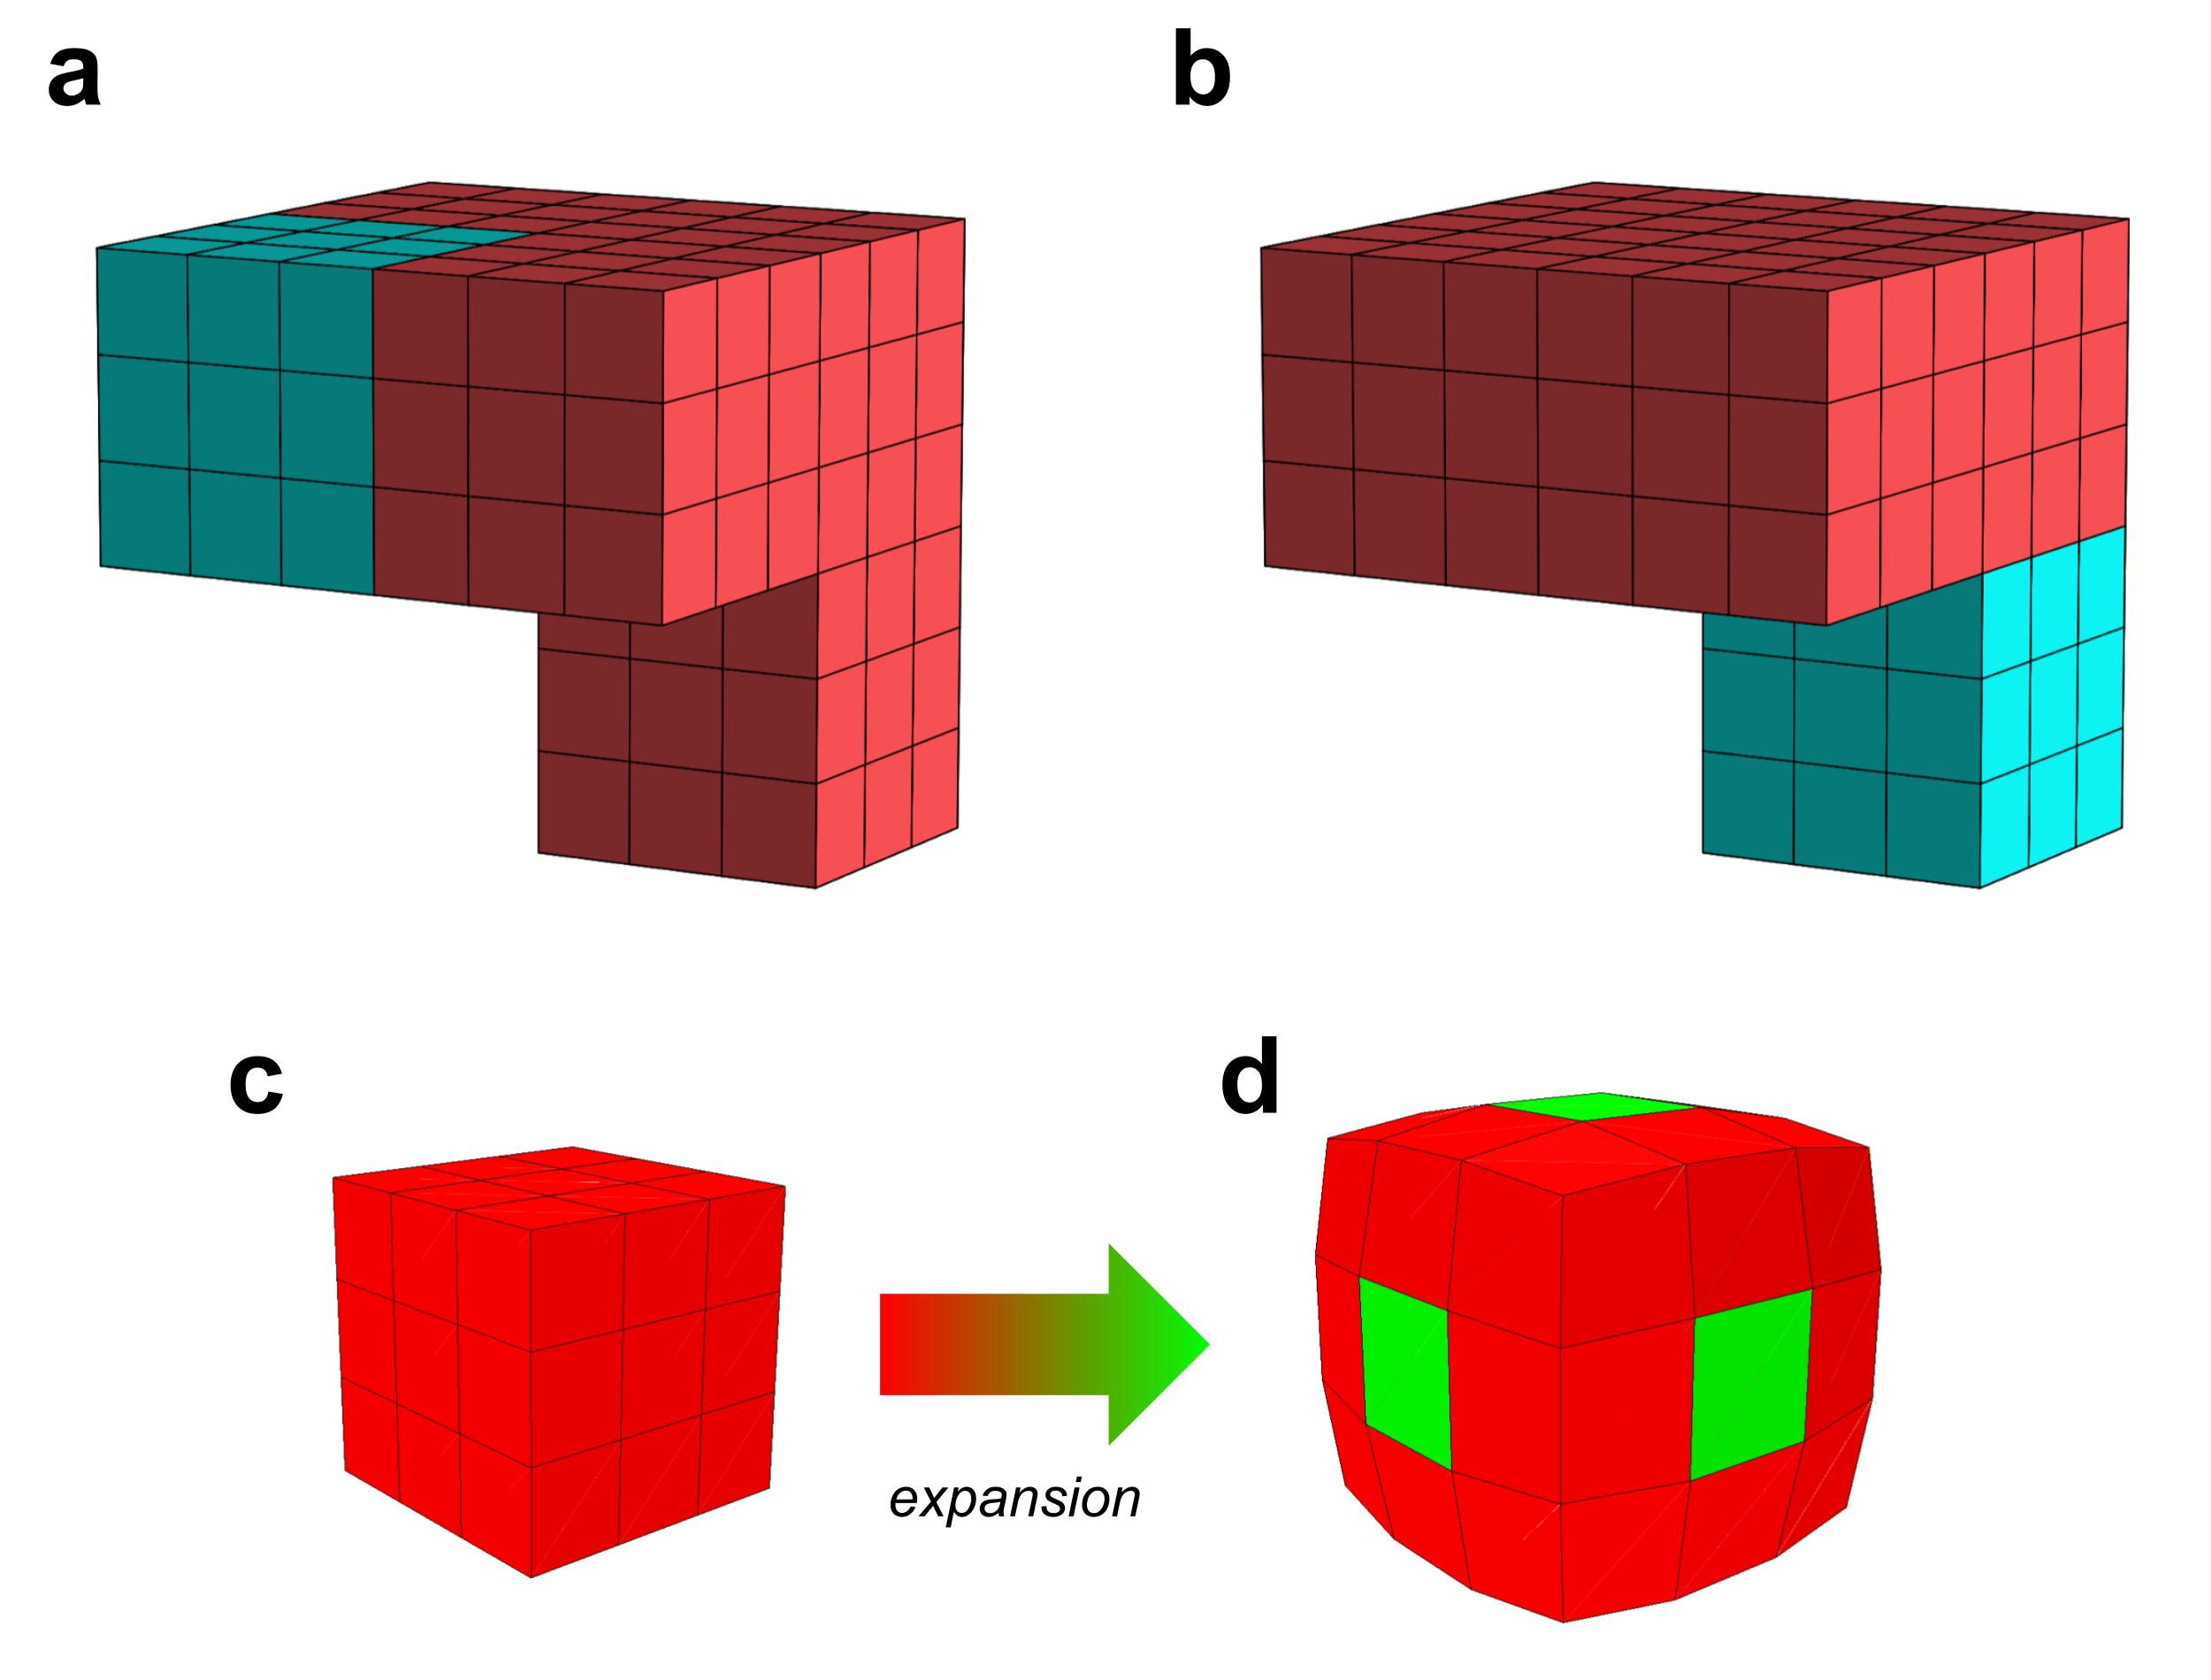
\includegraphics[width=0.65\linewidth]{Chapter02/fig/Yale_High_Res_Sim.jpg}
    % \vspace{-1em}
    \caption{A higher resolution model in which each silicone voxel is approximated by a 3-by-3-by-3 group of simulated subvoxels: a high-res voxel.
    The design in \textbf{a} and \textbf{b} are high-res instantiations of those in Figs.~\ref{fig:transfer}e and \ref{fig:transfer}f, respectively. 
    Spherical volumetric expansion in a high-res voxel (\textbf{c}) was approximated by increasing the rest length between the centermost subvoxel and the subvoxels at center of each face (green subvoxels in \textbf{d}).
    }
    \label{fig:hi_res_sim}
    % \vspace{-1.25em}
\end{figure}



\section{Discussion}
\label{sec:discussion}


In this paper, a new approach to robot damage recovery has been proposed.
Instead of presenting the remnant shape of the damaged robot to optimization as 
fixed,
we enable optimization to change this shape as the essential part of the recovery process.
In doing so we realized a machine that recovered more function than an otherwise equivalent system that could adapt its controller but not deform its shape.

In future work we will improve the transferal of simulated morphing machines
to physical ones using existing sim2real methods~\cite{bharadhwaj2018data, bongard2006resilient, cully2015robots, hwangbo2019learning, kwiatkowski2019task, tan2018sim} adapted appropriately to meet the additional
transferal demands dictated by soft materials~\cite{matas2018sim}. 
We will also generalize our optimization method
such that control and shape readaptation can be combined as dictated by the form of damage, predamage structure of the robot, and its task environment.

\subsection{Biological regeneration.}

In past work, rigid-bodied robots have been venerated for their ability to ``adapt like animals''~\cite{bongard2006resilient,cully2015robots}.
These machines, which were constructed from undeformable metals and hard plastics, 
automatically learned to control their bodies in spite of missing or broken legs.
But when an animal loses one or more of its legs to injury, it does not adapt by merely searching for a new mental representation of behavior that successfully maps onto the damaged body. 
Rather, they often fundamentally deform their damaged ``hardware'' into something more controllable.


Evidence for this abounds.
A famous example is the congenitally two-legged goat described by Slijper~\cite{slijper1942biologic}: 
an otherwise normal goat which was born without forelegs adopted an upright posture and learned to walk on its hind legs alone.
In addition to enlarged 
hind legs, 
striking changes in morphology were documented, including
a greatly elongated gluteal tongue and 
an innovative arrangement of small tendons,
a narrowed pelvis,
an oval (rather than V-shaped) thoracic cross-sectional shape,
a curved spine, 
and an unusually large neck~\cite{west2005developmental}.
The animal's body resembled that of a kangaroo more closely than that of a normal goat.


Other animals can regenerate.
The planarian flatworm can be cut into many pieces (the record is 279) all of which grow back to a full organism, regenerating not just tail and head, but eyes and the complete nervous system~\cite{montgomery1974minimal}.
Vertebrates, such as 
frogs, also display the capability of regenerating limbs, 
jaws, eyes and a variety of internal structures~\cite{brockes1997amphibian}. 
Humans too (especially children) are sometimes capable of fingertip regeneration after distal phalange amputation~\cite{illingworth1974trapped}. 

\subsection{Mechanisms of biological regeneration.}

Several of the mechanisms by which organisms achieve these forms of 
self-editing of their own anatomy pose design
challenges and future research directions for robotics.

First is the ability to harness the behavior of low-level components (cells) towards a specific large-scale goal-state: salamanders can regenerate whole limbs, eyes, tails, ovaries, and other organs \cite{mccusker2011axolotl},
but growth and remodeling ceases when a correctly shaped and sized organ is complete \cite{pezzulo2016top}.
Second is the flexibility and robustness of systems under novel conditions. For example, tadpoles whose facial organs are experimentally placed in abnormal configurations will undergo novel rearrangements to still give rise to normal frog faces during metamorphosis \cite{vandenberg2012normalized}, 
showing that the genome encodes not a hardwired set of movements for each organ but rather specifies a machine that can remodel toward the same target morphology from a variety of unexpected starting states. 
Thus, it is critical to understand and exploit the ability of evolution to give rise to hardware that is well-adapted to the normal environment but also retains significant plasticity \cite{sullivan2016physiological}. 

Third is the fact that during regeneration, the tissues making growth and morphogenesis decisions are themselves being drastically rearranged: thus, the computational control circuitry \textit{is itself} the object of the deformation actuators, forming a closed loop in which information is reliably processed in a medium that is constantly changing \cite{pezzulo2015re}. 
Finally, the remarkable robustness of morphological computation extends to information learned within the lifetime of the organism \cite{blackiston2015stability}.
Butterflies, which result from a caterpillar brain that is almost completely dissolved during metamorphosis, still remember information learned during the caterpillar stage \cite{blackiston2008retention}. 
Flatworms, which regrow their entire heads, still remember information they learned prior to decapitation \cite{corning1967regeneration, shomrat2013automated}. 

Attempts to implement these capabilities in artificial systems (whether robotic or via synthetic biology) are likely to enrich not only engineering technology, but also to feed back to the biological sciences and biomedicine. 
The current understanding of computation in biological tissues has numerous gaps, which are only likely to be filled by attempts to build these capabilities from the ground up \cite{kamm2018perspective}. 


\subsection{Metamorphosing machines.}

It has been shown here that robots, too, are not only capable of regenerating limbs, but that such deformation can manifest by selecting for function recovery alone, instead of a target legged shape.


However, this ability largely depends on the material with which robots are made, for even if morphology is free to change in rigid bodies, the ways in which such change can occur are limited at best.
In~\cite{bongard2011morphological}, robots used a combination of rotary and linear actuators to slowly angle appendages downward and extrude them outward, thus simulating limb growth.
In softer machines, there are more ways for morphology to change: 
The soft robot used here was able to locally deform its geometry to bend, twist, compress or expand throughout its body.
Its also possible, although not investigated here, for soft robots to change their material properties, such as stiffness, 
through (e.g.) granular jamming~\cite{brown2010universal,kriegman2018interoceptive}. 
% narang2018transforming,steltz2009jsel}. 


The possibility of this latter change highlights the inadequacy of the name ``soft robot''.
When a granular jamming robot jams (removes excess internal air to become stiff) does it cease to be a soft robot?
What if it never unjams?
For the purposes of damage repair, the most important property of soft robots is not that they are soft \textit{per se}, but that they may easily change their structural and material properties (possibly including stiffness).
One can envisage future ``rigid'' nanobots capable of self-assembling into a protean metamachine that can rearrange so as to regrow a lost part; but that day seems far off, whereas soft robots, capable of continuous morphological change, are already becoming a reality.


The future of this line of work promises not just new robotic systems but also new science. Shapeshifting robots, recast as scientific tools, can shed new light on old biological questions about developmental plasticity, regeneration and homeostasis~\cite{kriegman2017minimal,kriegman2018morphological,lobo2012modeling}.
And, symmetrically, new theories about the mechanisms that lie at the heart of such questions can be physically instantiated and optimized in a new breed of useful, autonomous and adaptive machines.





\section*{Acknowledgements}

This work was supported by 
NSF award EFRI-1830870 
and
DARPA contract HR0011-18-2-0022.
% D.~Shah was supported by 
% NASA STRF-80NSSC17K0164.
% G.~Branin was supported by an REU supplement to NSF award EFRI-1830870.





\renewcommand{\arraystretch}{1.3}
\setlength\tabcolsep{5pt}

\begin{table*}
\caption{\label{table:core_materials}The construction kit for making fifty 2-by-2-by-2 designs.}
\vspace{-1.5em}
\begin{scriptsize}
\begin{center}
\begin{tabular}{clcl} 
 \toprule
 \textbf{No.} & \textbf{Part} & \textbf{Cost} & \textbf{Notes} \\ 
 \toprule
 1 & Dragon Skin 10 FAST, 2 lbs kit (Smooth-On, Inc.) & \$32.21 & Created voxel bodies and connected x,y slices. \\ 
 \rowcolor{gray!25}
 2 & Sil-Poxy, 3 ounce tube (Smooth-On, Inc.) & \$30.72 & Secured tubing and repaired air leaks in six-sided voxels. \\ 
 3 & 1/32'' ID silicone tubing, 52 ft & \$34.32 & 50A shore hardness; connected voxels to actuation system. \\ 
 \rowcolor{gray!25}
 4 & 1/16'' pneumatic plastic connectors, 200 pieces & \$100 & Straight and T shaped. \\ 
 5 & 1/16'' ID silicone tubing, 65.6 ft & \$62.98 & 50A shore hardness; part of actuation system. \\ 
 \rowcolor{gray!25}
 6 & 60 mL Plastic Syringe (McMaster-Carr, Inc.) & \$3.13 &  Used to hand-actuate voxels while checking for leaks. \\
 \multirow{2}{*}{7} & \multirow{2}{22em}{1000 mL beaker (PYREX VISTA Griffin, Fisher Scientific International, Inc.)} & \multirow{2}{*}{\$14} & \multirow{2}{*}{Voxels were inflated in this beaker filled with water to detect leaks.} \\
  & & & \\ 
  \rowcolor{gray!25}
 8 & Hole punch 1/4 rectangle (Fiskars) & \$10.35 & Created holes between voxels within a slice so they actuated as a unit. \\ 
 9 & X-Acto Knife (McMaster-Carr, Inc.) & \$4.11 & Cut bottomless voxels out of acrylic mold, and trim the edges. \\ 
 \rowcolor{gray!25}
 10 & 100 mL mixing cups (VWR international), pack of 100 & \$66 & Where silicone was mixed. \\ 
 11 & Spatula (McMaster-Carr, Inc.) & \$7.50 & Spread the Dragon Skin on the edges of the acrylic mold. \\ 
 \rowcolor{gray!25}
 12 & 2 Scrap acrylic sheets, 12''$\times$12''$\times$1/8'' & \$10.58 & Collected scrap Dragon Skin; the surface where voxel bottom were created. \\ 
 13 & 2-1mm thick 30 cm metal rulers & \$6.99 & Used to set a thickness for sixth voxel side (bottom layer). \\ 
 \rowcolor{gray!25}
 14 & Double-sided tape & \$4.99 & Adhered the rulers to a scrap acrylic sheet. \\ 
 15 & Simple 30 cm metal ruler & \$3.99 & Spread a thin sheet of Dragon Skin onto scrap acrylic sheet for sixth side. \\ 
 \rowcolor{gray!25}
 16 & Popsicle stick (11.3 cm $\times$ 1 cm), box of 1000 & \$13.49 & Applied thin layer of silicone to bond adjacent voxels and x,y slices. \\ 
%  \multirow{2}{*}{17} & \multirow{2}{18em}{Cotton-tipped applicators, 6 inch (McKesson Corp.), box of 1000} & \multirow{2}{*}{\$8.99} & \multirow{2}{*}{Used to spread Sil-Poxy.} \\
%   & & \\ 
  17 & Cotton-tipped applicators, 6 inch, box of 1000 & \$8.99 & (McKesson Corp.) Used to spread Sil-Poxy. \\
  \rowcolor{gray!25}
 18 & Disposable Gloves (Halyard Inc.), box of 100 & \$8.95 & Wore when handling uncured silicone. \\ 
 19 & 2 Acrylic sheets, 12''$\times$12''$\times$1/8'' (McMaster-Carr, Inc.) & \$18.30 & Used to manufacture the open-face acrylic mold with laser-cut. \\ 
 \rowcolor{gray!25}
 20 & 41 mm binder clips, pack of 12 & \$7.99 & Held the acrylic mold onto the rotational molding machine. \\
 \toprule
  & \textbf{The rotational molding machine:} & & \\
 \toprule
 \rowcolor{gray!25}
 21 & Acrylic sheet, 12''$\times$12''$\times$1/4'' (McMaster-Carr, Inc.) & \$17.34 &  2$\times$ triangular plates, 3$\times$ motor mount - supports for rotational machine. \\ 
 22 & Acrylic sheet, 12''$\times$12''$\times$1/4'' (McMaster-Carr, Inc.) & \$17.34 & Mounting plate; holes were cut to minimize weight. \\ 
 \rowcolor{gray!25}
 23 & Pololu 4756 DC rotational motor & \$39.95 & Used for rotational molding machine. \\ 
 24 & Pololu 1999 mounting hum  & \$7.95 & Used to mount rotational molding machine. \\ 
 \rowcolor{gray!25}
 25 & Arduino Uno Microcontroller & \$22 & Controlled rotation timing and degree. \\ % https://store.arduino.cc/usa/arduino-uno-rev3
 25 & Arduino Motor Shield  & \$19.95 & Controlled rotation motor. \\  % https://www.adafruit.com/product/1438
 \rowcolor{gray!25}
 26 & AC charger & \$10.42 & 12mm$\times$2.1$\times$5.5mm barrel jack, 12V, Supplies power to the Arduino. \\ 
 27 & 8020 T-Slotted Solid 1'' beams (McMaster-Carr, Inc.) & \$12.31 & 2$\times$10 cm, 2$\times$40 cm, Supports for rotational molding machine. \\ 
 \rowcolor{gray!25}
 28 & 8020 screws and T-nuts & \$7.92 & Connected 8020 beams. \\ % 14 of product 3382, 14 of product 3061 
 29 & ``M3$\times$10'' screws & \$1.24 & Used to mount rotational molding machine. \\ 
 \rowcolor{gray!25}
 30 & Irwin QuickGrip 12''$\times$2.75'' Clamp & \$15.99 & Held rotational molding machine to table. \\
 \toprule
  & \textbf{Grand total:} & \textbf{\$622} &  \\
 \bottomrule
\end{tabular}
\end{center}
\end{scriptsize}
\vspace{-2.5em}
\end{table*}


\bibliographystyle{plainnat}
\bibliography{main}



\end{document}


